%%=============================================================================
%% Methodologie
%%=============================================================================

\chapter{\IfLanguageName{dutch}{Methodologie}{Methodology}}%
\label{ch:methodologie}

\section{Methodologie}%
\label{sec:methodologie}

Dit hoofdstuk beschrijft op hoofdlijnen hoe het onderzoek werd opgezet en uitgevoerd. Het doel van de methodologie is een reproduceerbaar proces te beschrijven waarmee verschillende LLM's systematisch kunnen worden geëvalueerd op de kwaliteit van hun Python code voor data analyse en ETL taken. Het onderzoeksontwerp is geïnspireerd door bestaande evaluatiekaders voor LLM codegeneratie, waarin een verzameling van programmeerproblemen wordt gekoppeld aan een volledig geautomatiseerde evaluatiepipeline die de gegenereerde code systematisch beoordeelt op zeven kwaliteitsdimensies \autocite{Li2023,Ni2024,LopezEspejel2025}. De eigenlijke verzameling van taken, de gedetailleerde resultaten en de codevoorbeelden worden verder uitgewerkt in de daaropvolgende hoofdstukken. In dit hoofdstuk wordt een concreet overzicht gegeven van de gekozen casussen, de gebruikte prompts, de inputdata, de verwachte output en de gehanteerde evaluatiemethode. 

\section{Fase 1: Literatuurstudie en afbakening van het takenpakket}

De eerste fase bestond uit een gerichte literatuurstudie naar de betrouwbaarheid van LLM gegenereerde code, bestaande benchmarks en evaluatiemetrics voor codegeneratie en typische data analyse en ETL taken in Python die relevant zijn voor studenten Toegepaste Informatica \autocite{Li2023,Esfahani2024,Ni2024}. Op basis van deze studie werden de kwaliteitscriteria voor de evaluatie afgebakend. De code werd beoordeeld op syntactische correctheid, semantische correctheid, beveiliging, uitvoerbaarheid, performantie, complexiteit, onderhoudbaarheid en functionele correctheid.

De deliverable in deze fase is een duidelijk gedefinieerd takenpakket van 35 representatieve Python opdrachten die typische data engineering activiteiten weerspiegelen. Deze opdrachten werden verdeeld over 8 categorieën: data cleaning, data transformation, joins en aggregation, performance optimization, data loading, data validation, data filtering en time series. Voor elke casus werden een natuurlijke taalprompt, inputdata en verwachte output geformuleerd, in lijn met de manier waarop codegeneratiebenchmarks zoals HumanEval en vergelijkbare studies hun problemen structureren \autocite{Ni2024,LopezEspejel2025}. Deze casussen vormen de basis voor de latere volledig geautomatiseerde evaluatie via de pipeline.

\subsection{Overzicht van de casuscategorieën}

De 35 evaluatiecasussen werden als volgt verdeeld:

\begin{itemize}
    \item 7 casussen rond data cleaning.
    \item 6 casussen rond data transformation.
    \item 5 casussen rond joins en aggregation.
    \item 4 casussen rond performance optimization.
    \item 2 casussen rond data loading.
    \item 5 casussen rond data validation.
    \item 5 casussen rond data filtering.
    \item 1 casus rond time series.
\end{itemize}

Deze verdeling werd gekozen om zowel veelvoorkomende als iets complexere data engineering scenario's af te dekken.

\subsection{Voorbeeldcasussen}

Onderstaande voorbeelden illustreren hoe de casussen zijn opgebouwd. Elke casus bestaat uit een prompt, een inputbestand, een verwachte output en een selectie van evaluatiecriteria. De inputdata voor de evaluatiecasussen bestaat uit realistische CSV-bestanden die afkomstig zijn van een concreet project: een aanwezigheidstracking systeem voor studenten op basis van WiFi-netwerklogin. Deze dataset bevat loggegevens van studenten die inloggen op het universitaire WiFi-netwerk, met velden zoals timestamp, gebruikersID, apparaattype en sessieduur. Door gebruik te maken van deze authentieke, real-world data in plaats van synthetisch gegenereerde testbestanden, wordt de validiteit van de evaluatie vergroot en worden de modellen getest op scenario's die nauw aansluiten bij daadwerkelijke data engineering taken.

\subsubsection*{Casus 1: Missing Value Imputation}

\textbf{Categorie:} Data Cleaning

\textbf{Prompt:} Schrijf een Python script dat een CSV bestand inleest en missing values behandelt. Vul numerieke kolommen met het gemiddelde, categorische kolommen met de modus. Sla op naar output.csv.

\textbf{Inputdata:} \texttt{input.csv} met de kolommen \texttt{name}, \texttt{age} en \texttt{city}, waarbij enkele \texttt{age} en \texttt{city} waarden ontbreken.

\textbf{Verwachte output:}
\begin{itemize}
    \item Numerieke kolom \texttt{age} heeft missing values ingevuld met het gemiddelde.
    \item Categorische kolom \texttt{city} heeft missing values ingevuld met de modus.
    \item Het resultaatbestand bevat geen null waarden meer.
\end{itemize}

\textbf{Geteste criteria:} syntax, semantische correctheid, uitvoerbaarheid, functional correctness.

\subsubsection*{Casus 2: Duplicate Removal}

\textbf{Categorie:} Data Cleaning

\textbf{Prompt:} Schrijf een Python script dat duplicaten verwijdert op basis van de combinatie \texttt{user\_id} en \texttt{order\_id}. Behoud de rij met de nieuwste timestamp. Sla op naar output.csv.

\textbf{Inputdata:} \texttt{input.csv} met vier rijen, waaronder één duplicaat op basis van \texttt{user\_id} en \texttt{order\_id}.

\textbf{Verwachte output:}
\begin{itemize}
    \item Exact drie rijen in de output.
    \item Correcte verwerking van datetime waarden.
    \item De rij met de meest recente timestamp wordt bewaard.
\end{itemize}

\textbf{Geteste criteria:} syntax, semantische correctheid, uitvoerbaarheid, functional correctness.

\subsubsection*{Casus 3: Gemengde numerieke formaten}

\textbf{Categorie:} Data Cleaning, edge case

\textbf{Prompt:} Schrijf een Python script dat gemixte numerieke formaten opschoont. Verwijder \texttt{\$} en komma's uit \texttt{price}, verwijder \texttt{\%} uit \texttt{percentage}. Converteer alles naar \texttt{float}.

\textbf{Inputdata:} \texttt{input.csv} met waarden zoals \texttt{\$1,250.00}, \texttt{50\%}.

\textbf{Verwachte output:}
\begin{itemize}
    \item \texttt{price} wordt geconverteerd naar \texttt{float}.
    \item \texttt{percentage} wordt geconverteerd naar een numerieke waarde.
    \item \texttt{temperature} wordt geconverteerd naar \texttt{float}.
\end{itemize}

\textbf{Geteste criteria:} syntax, semantische correctheid, uitvoerbaarheid, functional correctness, edge case handling.

\subsubsection*{Casus 4: Null-achtige waarden}

\textbf{Categorie:} Data Cleaning, edge case

\textbf{Prompt:} Schrijf een Python script dat null-achtige waarden behandelt. \texttt{N/A}, \texttt{null}, \texttt{NULL}, \texttt{NaN}, \texttt{-} en lege strings worden allemaal als missing values beschouwd en geconverteerd naar echte \texttt{NaN} waarden.

\textbf{Inputdata:} \texttt{input.csv} met verschillende null-achtige representaties.

\textbf{Verwachte output:}
\begin{itemize}
    \item Alle null-achtige waarden worden geconverteerd naar echte missing values.
    \item Missing leeftijden worden aangevuld met het gemiddelde.
    \item Rijen met lege steden worden verwijderd.
\end{itemize}

\textbf{Geteste criteria:} syntax, semantische correctheid, uitvoerbaarheid, functional correctness, edge case handling.



\section{Fase 2: Opzetten van de automatische evaluatiepipeline}

In de tweede fase werd een automatische evaluatiepipeline ontwikkeld die de kern van het onderzoek vormt. Deze pipeline volgt conceptueel dezelfde driedelige structuur als voorgestelde frameworks voor code evaluatie: probleemvoorbereiding, modeluitvoering en codeanalyse \autocite{Li2023,LopezEspejel2025}. Alle taken en bijbehorende tests werden geïmplementeerd in Python, met gebruik van een testframework voor functionele verificatie.

De uitvoering van de verschillende LLM's gebeurde lokaal via Ollama, zodat meerdere modellen op een uniforme manier konden worden aangesproken zonder voor elk model een aparte integratie te moeten ontwikkelen. De geteste modellen waren: DeepSeek Coder V2 (deepseek-coder-v2:latest), Gemma 4 (gemma4:latest), Mistral (mistral:latest), Llama 3 (llama3:latest), Qwen 2.5 Coder (qwen2.5-coder:latest) en Phi 4 Mini (phi4-mini:latest). Voor elk model en elke taak genereerde de pipeline drie oplossingen door dezelfde prompt drie keer aan het model aan te bieden, zodat ook de variabiliteit tussen runs kon worden geanalyseerd. De gegenereerde code werd automatisch opgeslagen als aparte Python bestanden, waarna de pipeline voor elke oplossing de volgende stappen doorliep:

\begin{itemize}
\item syntaxiscontrole via AST parsing;
\item semantische en style controle via Ruff;
\item security analyse via Bandit;
\item meting van uitvoeringstijd, CPU gebruik en geheugenverbruik tijdens executie op een vaste dataset;
\item analyse van complexiteit en onderhoudbaarheid via Radon wat een Python tool is die statische codeanalyse uitvoert om metrische waarden zoals cyclomatische complexiteit, maintainability index en codekwaliteit van Python code te meten;
\item functionele tests om te controleren of de verwachte output correct werd gegenereerd.
\end{itemize}

De resultaten van deze automatische evaluatie, bijvoorbeeld geslaagd of niet geslaagd, aantal tests geslaagd en type fouten, werden gestructureerd opgeslagen in een JSON formaat zodat latere analyse mogelijk bleef. De deliverable van deze fase is een werkende, volledig geautomatiseerde evaluatieomgeving die meerdere modellen en runs zonder menselijke tussenkomst kan verwerken, vergelijkbaar met de automatische processen die in recente evaluatiestudies worden voorgesteld \autocite{Li2023,LopezEspejel2025}. De volledige code van de evaluatiepipeline, inclusief alle scripts, prompts en testdata, is openbaar beschikbaar via de GitHub repository: \url{https://github.com/renaudVermeiren/Onderzoek}.

\subsection{Keuze voor lokale open-source modellen}

De keuze om lokaal draaiende open-source modellen te gebruiken via Ollama is bewust gemaakt op basis van vier argumenten die zowel de wetenschappelijke kwaliteit als de praktische uitvoerbaarheid van dit onderzoek ondersteunen.

Een eerste overweging is reproduceerbaarheid. Commerciële API's zoals ChatGPT of Copilot kunnen hun modelversies, parameters of beschikbaarheid wijzigen zonder voorafgaande kennisgeving, waardoor het moeilijk is om een experiment exact te herhalen. Door open source modellen lokaal te draaien heb ik volledige controle over de exacte modelversie, configuratie en uitvoeringsomgeving, wat essentieel is voor een reproduceerbare benchmark.

Ten tweede speelt kostenefficiëntie een rol. Een vergelijkend experiment met zes modellen, 35 taken en drie runs per taak levert 630 individuele codegeneraties op. Bij commerciële API's zou dit aanzienlijke kosten met zich meebrengen, terwijl lokale uitvoering op eigen hardware deze drempel wegneemt en het mogelijk maakt om grootschaliger te experimenteren zonder kosten beperkingen.

Een derde argument is privacy en het kunnen beheren van je eigen data. Omdat de prompts en gegenereerde code binnen de evaluatiepipeline soms voorbeeld datasets, bestandsnamen of hypothetische scenario's bevatten, blijven deze gegevens bij lokale uitvoering volledig binnen de eigen omgeving.

Tot slot is de keuze voor Ollama als uniforme interface praktisch omdat het model onafhankelijke vergelijking voorziet. Zonder Ollama zou voor elk model een aparte API integratie nodig zijn, wat de complexiteit van de pipeline zou verhogen en de kans op implementatieverschillen tussen modellen zou introduceren. Door alle modellen via dezelfde lokale interface aan te spreken, worden externe variabelen zoveel mogelijk geëlimineerd, waardoor de geobserveerde prestatieverschillen beter toegeschreven kunnen worden aan de modellen zelf.

\subsection{Scope en beperkingen}

Hoewel prompt engineering een belangrijk onderwerp is voor het begrijpen van LLM output \autocite{Guo2024,Yuen2025}, valt een systematische vergelijking van verschillende promptstrategieën buiten de scope van dit onderzoek. Deze bachelorproef richt zich op de evaluatie van gegenereerde codekwaliteit per model, gebruikmakend van gestandaardiseerde, natuurlijke taalprompts zonder expliciete promptingtechnieken zoals few shot, chain of thought of rolgebaseerde instructies. De keuze voor uniforme prompts maakt het mogelijk om de modellen onder gelijke omstandigheden te vergelijken, maar betekent tegelijk dat de resultaten niet generaliseren naar andere promptformuleringen of strategieën. Dit vormt een beperking van het onderzoek die relevant is voor de interpretatie van de resultaten en voor het ontwerp van toekomstig onderzoek.

\section{Fase 3: Vergelijking van modellen}

In de derde fase werden de verzamelde gegevens systematisch geanalyseerd per model, per taak, per evaluator en over de drie runs heen. De analyse volgt de rapporteringswijze van vergelijkende studies naar codegeneratieprestaties, met aandacht voor succesratio's, variabiliteit tussen runs en kwaliteitsverschillen per evaluatiedimensie \autocite{Li2023,Ni2024}. De evaluatie gebeurde volledig geautomatiseerd via de zeven evaluatiecriteria uit de pipeline, zonder manuele beoordeling. Voor elk model werden de volgende grootheden berekend:
\begin{itemize}
    \item \textbf{Pass rate per evaluator}: het percentage samples (van 105 totaal per model) dat slaagde voor Syntax, Style, Security, Execution, Performance, Radon wat een Python tool is die statische codeanalyse uitvoert om metrische waarden zoals cyclomatische complexiteit, maintainability index en codekwaliteit van Python code te meten en Functional;
    \item \textbf{Gemiddelde kwaliteitsscore}: het gemiddelde van alle evaluator scores (exclusief Functional) over alle taken, gebruikt voor de overall ranking;
    \item \textbf{Consistentie over runs}: de variabiliteit tussen de drie samples per taak, als indicator voor betrouwbaarheid van de codegeneratie;
    \item \textbf{Prestatie per taakcategorie}: de gemiddelde scores voor Data Cleaning, Data Transformation, Joins \& Aggregation, Performance Optimization en Data Operations;
    \item \textbf{Verdeling van code omvang en uitvoeringstijd}: statistische samenvatting (mediaan, interkwartielafstand) van regels code en executietijd.
\end{itemize}

Deze resultaten werden visueel samengevat in tabellen en grafieken en vormden de basis voor de beantwoording van de onderzoeksvraag en deelvragen. Parallel hiermee werd op basis van de geobserveerde patronen een praktisch evaluatiekader ontwikkeld, dat bestaat uit aanbevelingen voor teststrategieën bij data analyse en ETL taken en richtlijnen voor het kiezen en gebruiken van modellen via Ollama in een onderwijscontext. De deliverables van deze fase zijn de geanalyseerde resultaten en de daaruit afgeleide aanbevelingen. Deze opbouw sluit aan bij eerdere raamwerken in de literatuur, maar is specifiek afgestemd op Python gebaseerde data engineering taken en op de praktijkcontext van HOGENT \autocite{LopezEspejel2025}.

\section{Samenvatting van de onderzoekscasussen}

De 35 casussen dekken samen alle data engineering aspecten uit hoofdstuk 2 als concrete benchmarks. Per casus worden zowel functionele correctheid als codekwaliteit getest, met specifieke aandacht voor syntax, semantiek, security, performantie en onderhoudbaarheid. Door de casussen expliciet te koppelen aan prompts, inputdata en verwachte output ontstaat een reproduceerbare onderzoeksopzet waarmee de prestaties van verschillende LLM's objectief kunnen worden vergeleken. 

\begin{itemize}
\item \textbf{Syntax:} controle via AST parsing.
\item \textbf{Semantische correctheid:} controle via Ruff, wat een snelle Python-linter en formatter is die code controleert op fouten, stijlproblemen en kwaliteitsregels om consistente en propere Python code te garanderen.
\item \textbf{Security:} controle via Bandit, wat een beveiligingsgerichte Python-analysetool is die broncode scant op mogelijke kwetsbaarheden en onveilige programmeerpraktijken, zoals hardcoded wachtwoorden, gevaarlijke functies of onveilige bestands- en subprocess-aanroepen.
\item \textbf{Execution:} controle via runtime tests.
\item \textbf{Performance:} controle via CPU en geheugengebruik.
\item \textbf{Radon:} controle van complexiteit en onderhoudbaarheid.
\item \textbf{Functional:} controle van de verwachte output.
\end{itemize}

Deze aanpak levert een representatief beeld op van welk LLM model de beste code genereert voor realistische data engineering taken, en laat tegelijk toe om te analyseren in welke situaties modellen falen of extra begeleiding nodig hebben.



\subsection{Resultaten}
\label{subsec:resultaatvisualisatie}

De evaluatie omvatte zes modellen die elk op 35 ETL-taken werden getest, met drie samples per taak. Dit resulteerde in 630 individuele code-evaluaties. De resultaten worden gevisualiseerd in de volgende figuren.

\textbf{Figuur \ref{fig:01_evaluator_comparison}} toont een gegroepeerd staafdiagram van het gemiddelde slagingspercentage per evaluator voor elk model. \texttt{qwen2.5-coder} behaalde een perfecte score voor style (100\%) en excelleerde in syntax, security en Radon, maar bleef steken op 57,1\% voor functionele correctheid. \texttt{deepseek-coder-v2} toonde eveneens sterke syntactische en security-resultaten met een functionele score van 57,1\%. \texttt{gemma4} had de hoogste functionele score (58,1\%) maar de laagste style compliance (54,3\%). \texttt{llama3} scoorde hoog op overall quality (96,1\%) maar liet lagere scores zien voor execution (62,9\%) en functionaliteit (41,0\%). \texttt{phi4-mini} en \texttt{mistral} scoorden lager op functionaliteit, respectievelijk 36,2\% en 29,5\%.

\textbf{Figuur \ref{fig:task_performance}} visualiseert de gemiddelde kwaliteitsscore per taakcategorie. De modellen presteerden over het algemeen vergelijkbaar over de verschillende categorieën (Data Cleaning, Data Operations, Data Transformation, Joins \& Aggregation, Performance Optimization), met lichte variaties afhankelijk van de taakcomplexiteit.

\textbf{Figuur \ref{fig:maintainability}} toont de onderhoudbaarheidsindex (Radon) per model. Alle modellen scoorden uitstekend, met waarden boven de 95\%, wat erop wijst dat de gegenereerde code over het algemeen goed gestructureerd en leesbaar is.

\textbf{Figuur \ref{fig:lines_of_code}} geeft een boxplot-weergave van de code-omvang per model. Deze figuur toont de verspreiding in de lengte van de gegenereerde scripts, met de mediaan en de interkwartielafstand.

\textbf{Figuur \ref{fig:execution_times}} toont de verdeling van de uitvoeringstijden per model. Dit geeft inzicht in de runtime-efficiëntie van de gegenereerde code.

\textbf{Figuur \ref{fig:model_ranking}} presenteert de algemene rangschikking op basis van de gemiddelde kwaliteitsscore over alle evaluatoren (exclusief functionaliteit). De rangschikking is: \texttt{llama3} (96,1\%), \texttt{deepseek-coder-v2} (95,7\%), \texttt{qwen2.5-coder} (95,6\%), \texttt{mistral} (94,6\%), \texttt{phi4-mini} (89,0\%) en \texttt{gemma4} (86,9\%).

\textbf{Figuur \ref{fig:08_sample_consistency}} toont de consistentie over de drie samples per evaluator. Een lagere variantie wijst op een betrouwbaardere codegeneratie.

\textbf{Figuur \ref{fig:09_generation_speed}} toont de generatiesnelheid in tokens per seconde voor elk model.

\begin{figure}[htbp]
    \centering
    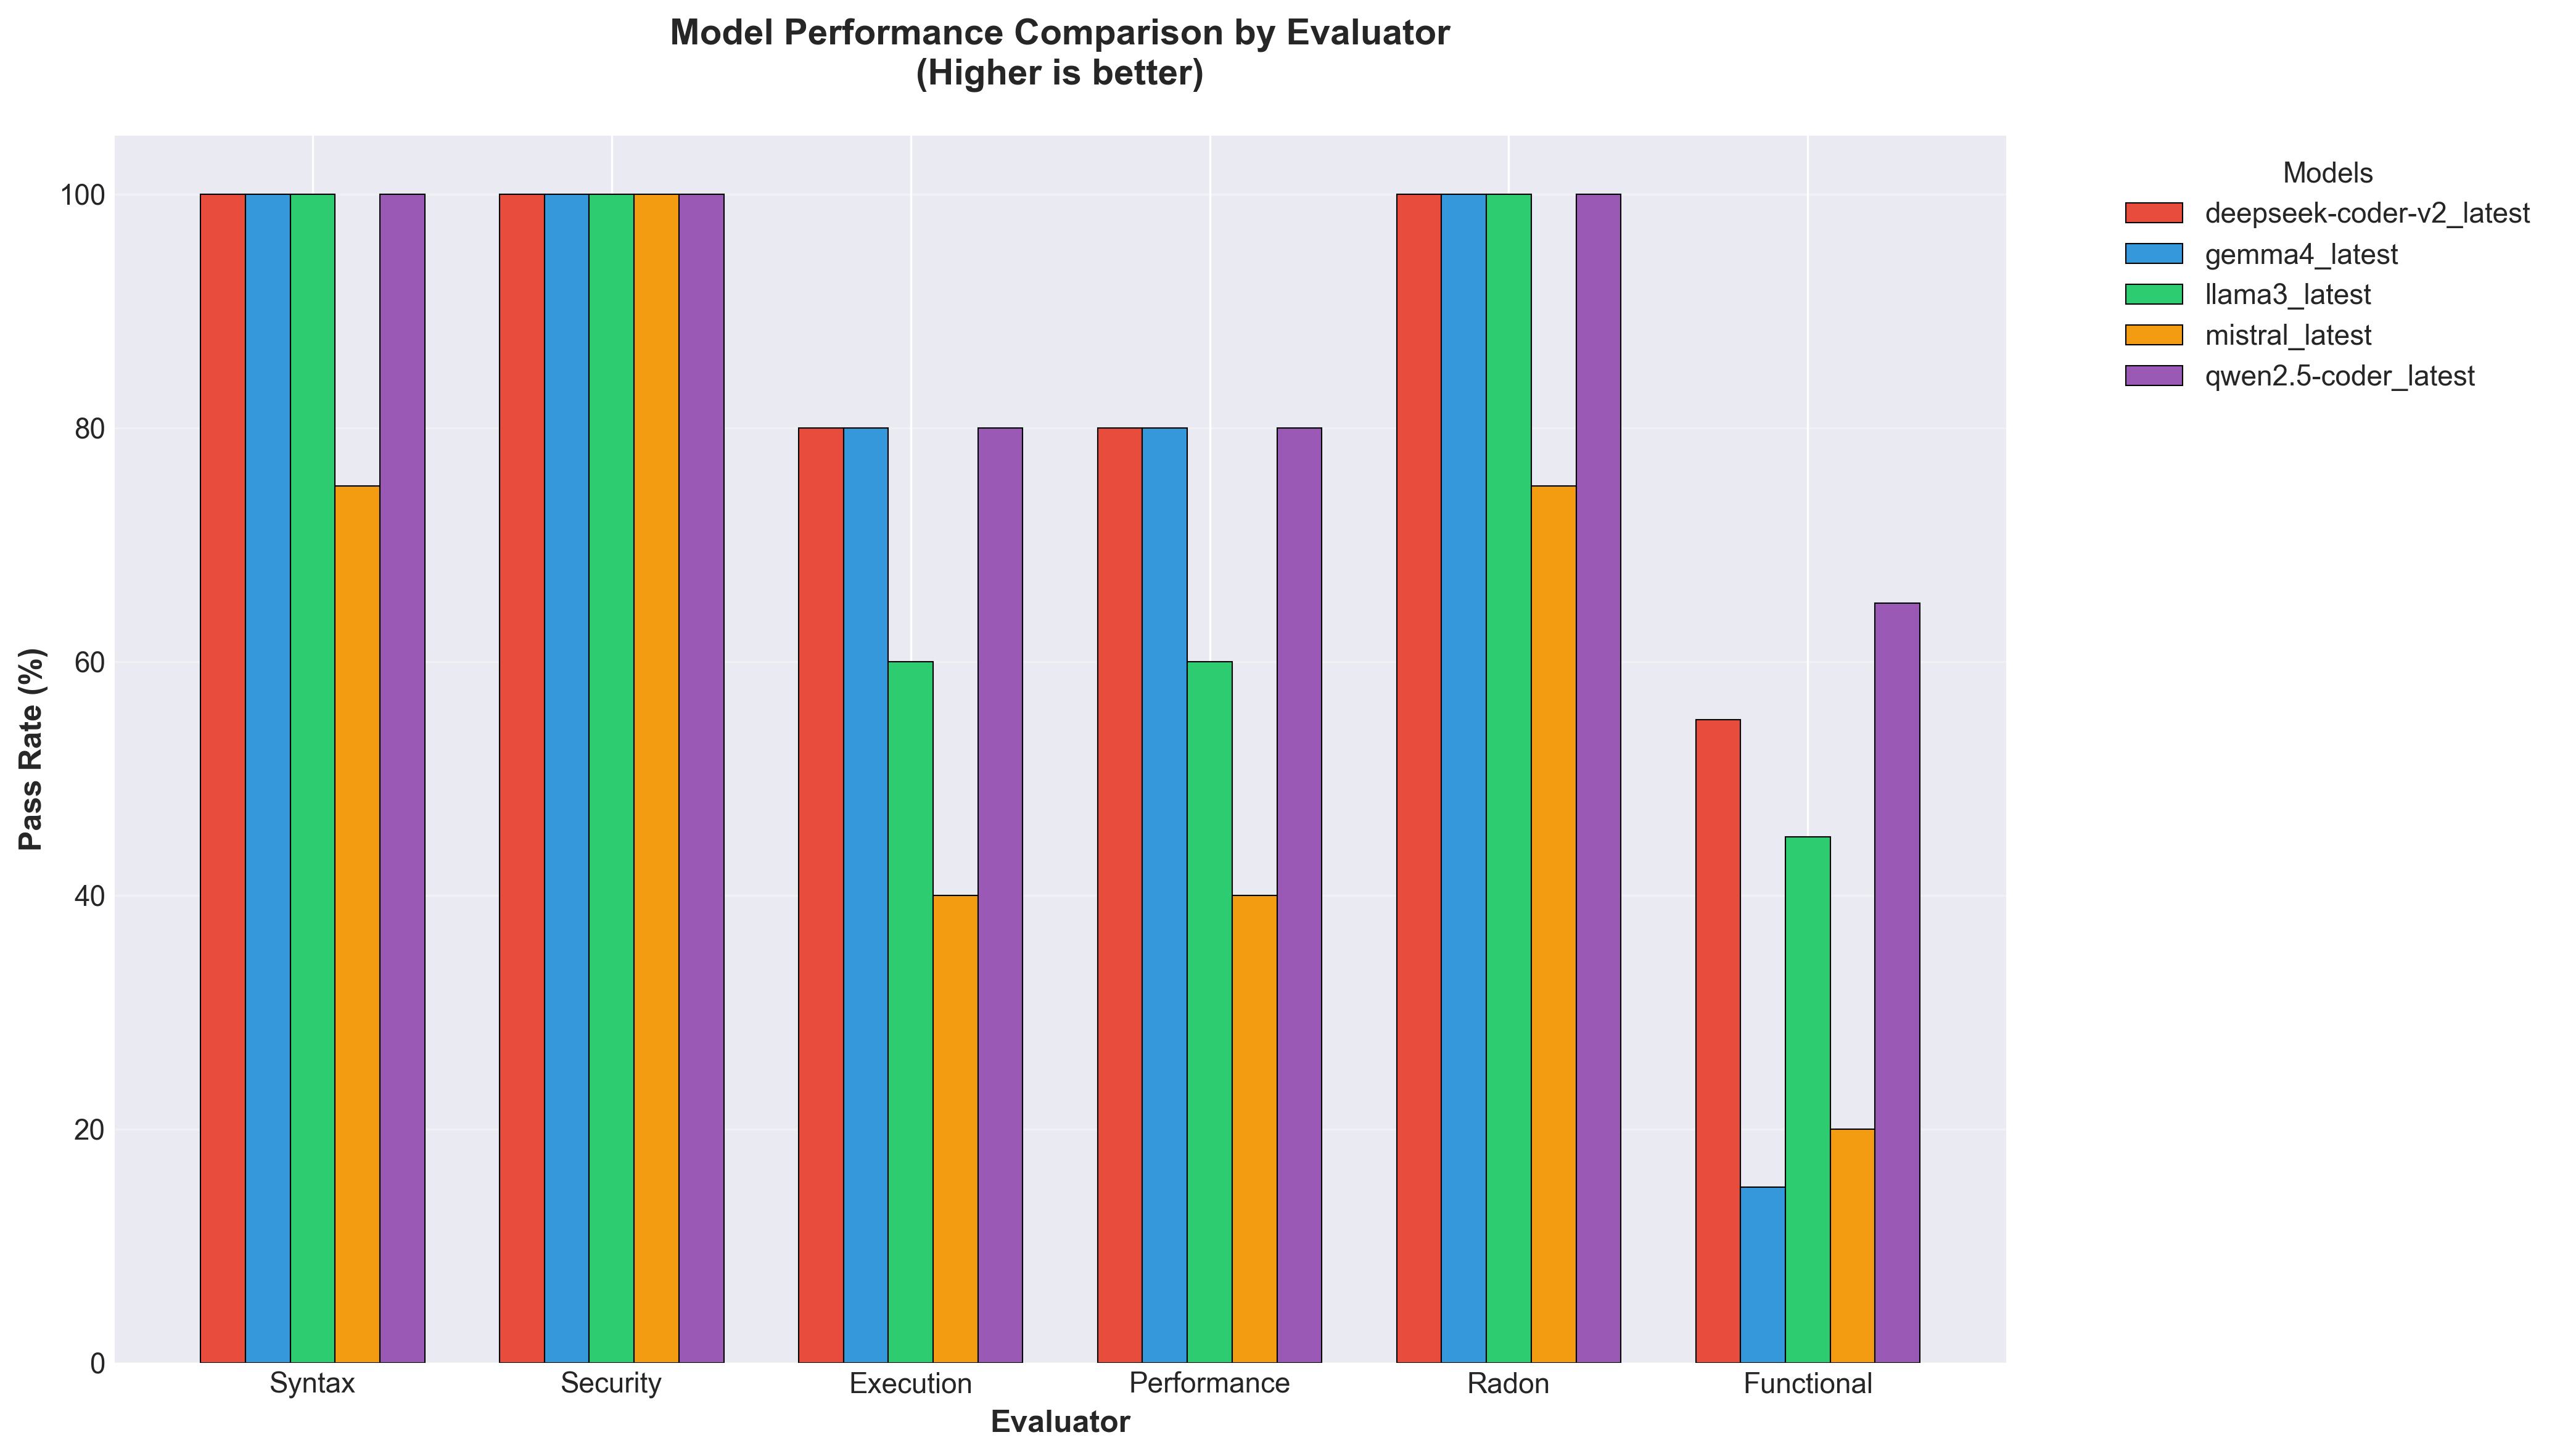
\includegraphics[width=0.9\linewidth]{images/01_evaluator_comparison.png}
    \caption{Vergelijking van de evaluatieresultaten per model.}
    \label{fig:01_evaluator_comparison}
\end{figure}

\begin{figure}[htbp]
    \centering
    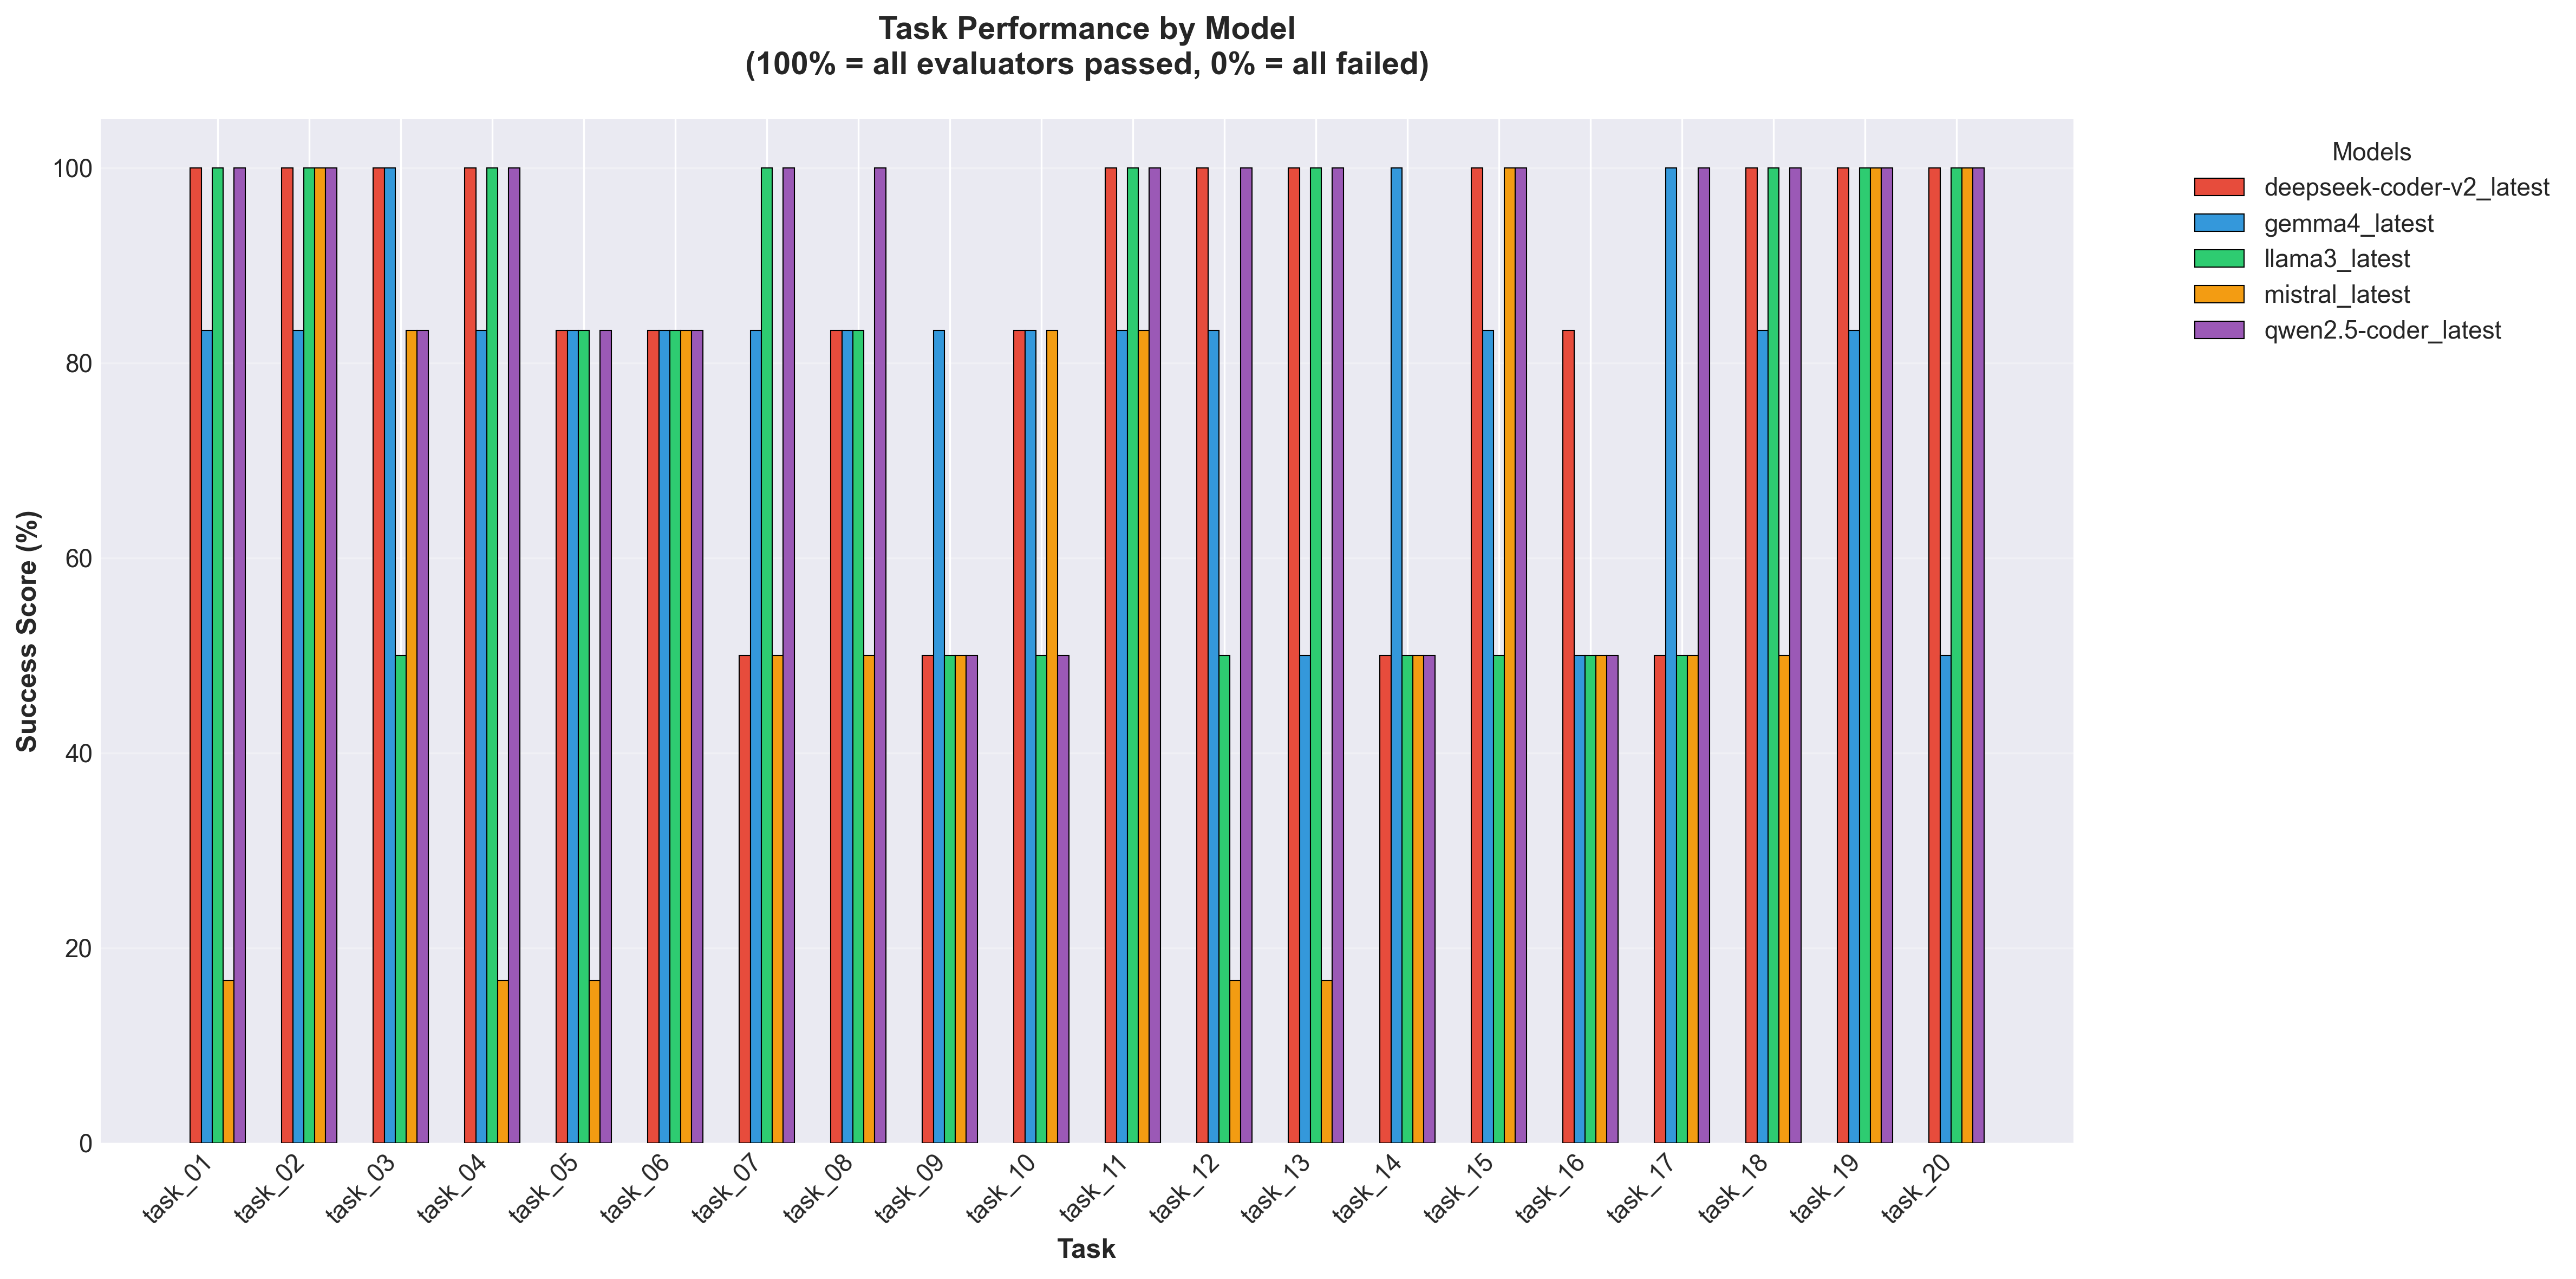
\includegraphics[width=0.9\linewidth]{images/02_task_performance.png}
    \caption{Prestatie van de modellen per taak.}
    \label{fig:task_performance}
\end{figure}

\begin{figure}[htbp]
    \centering
    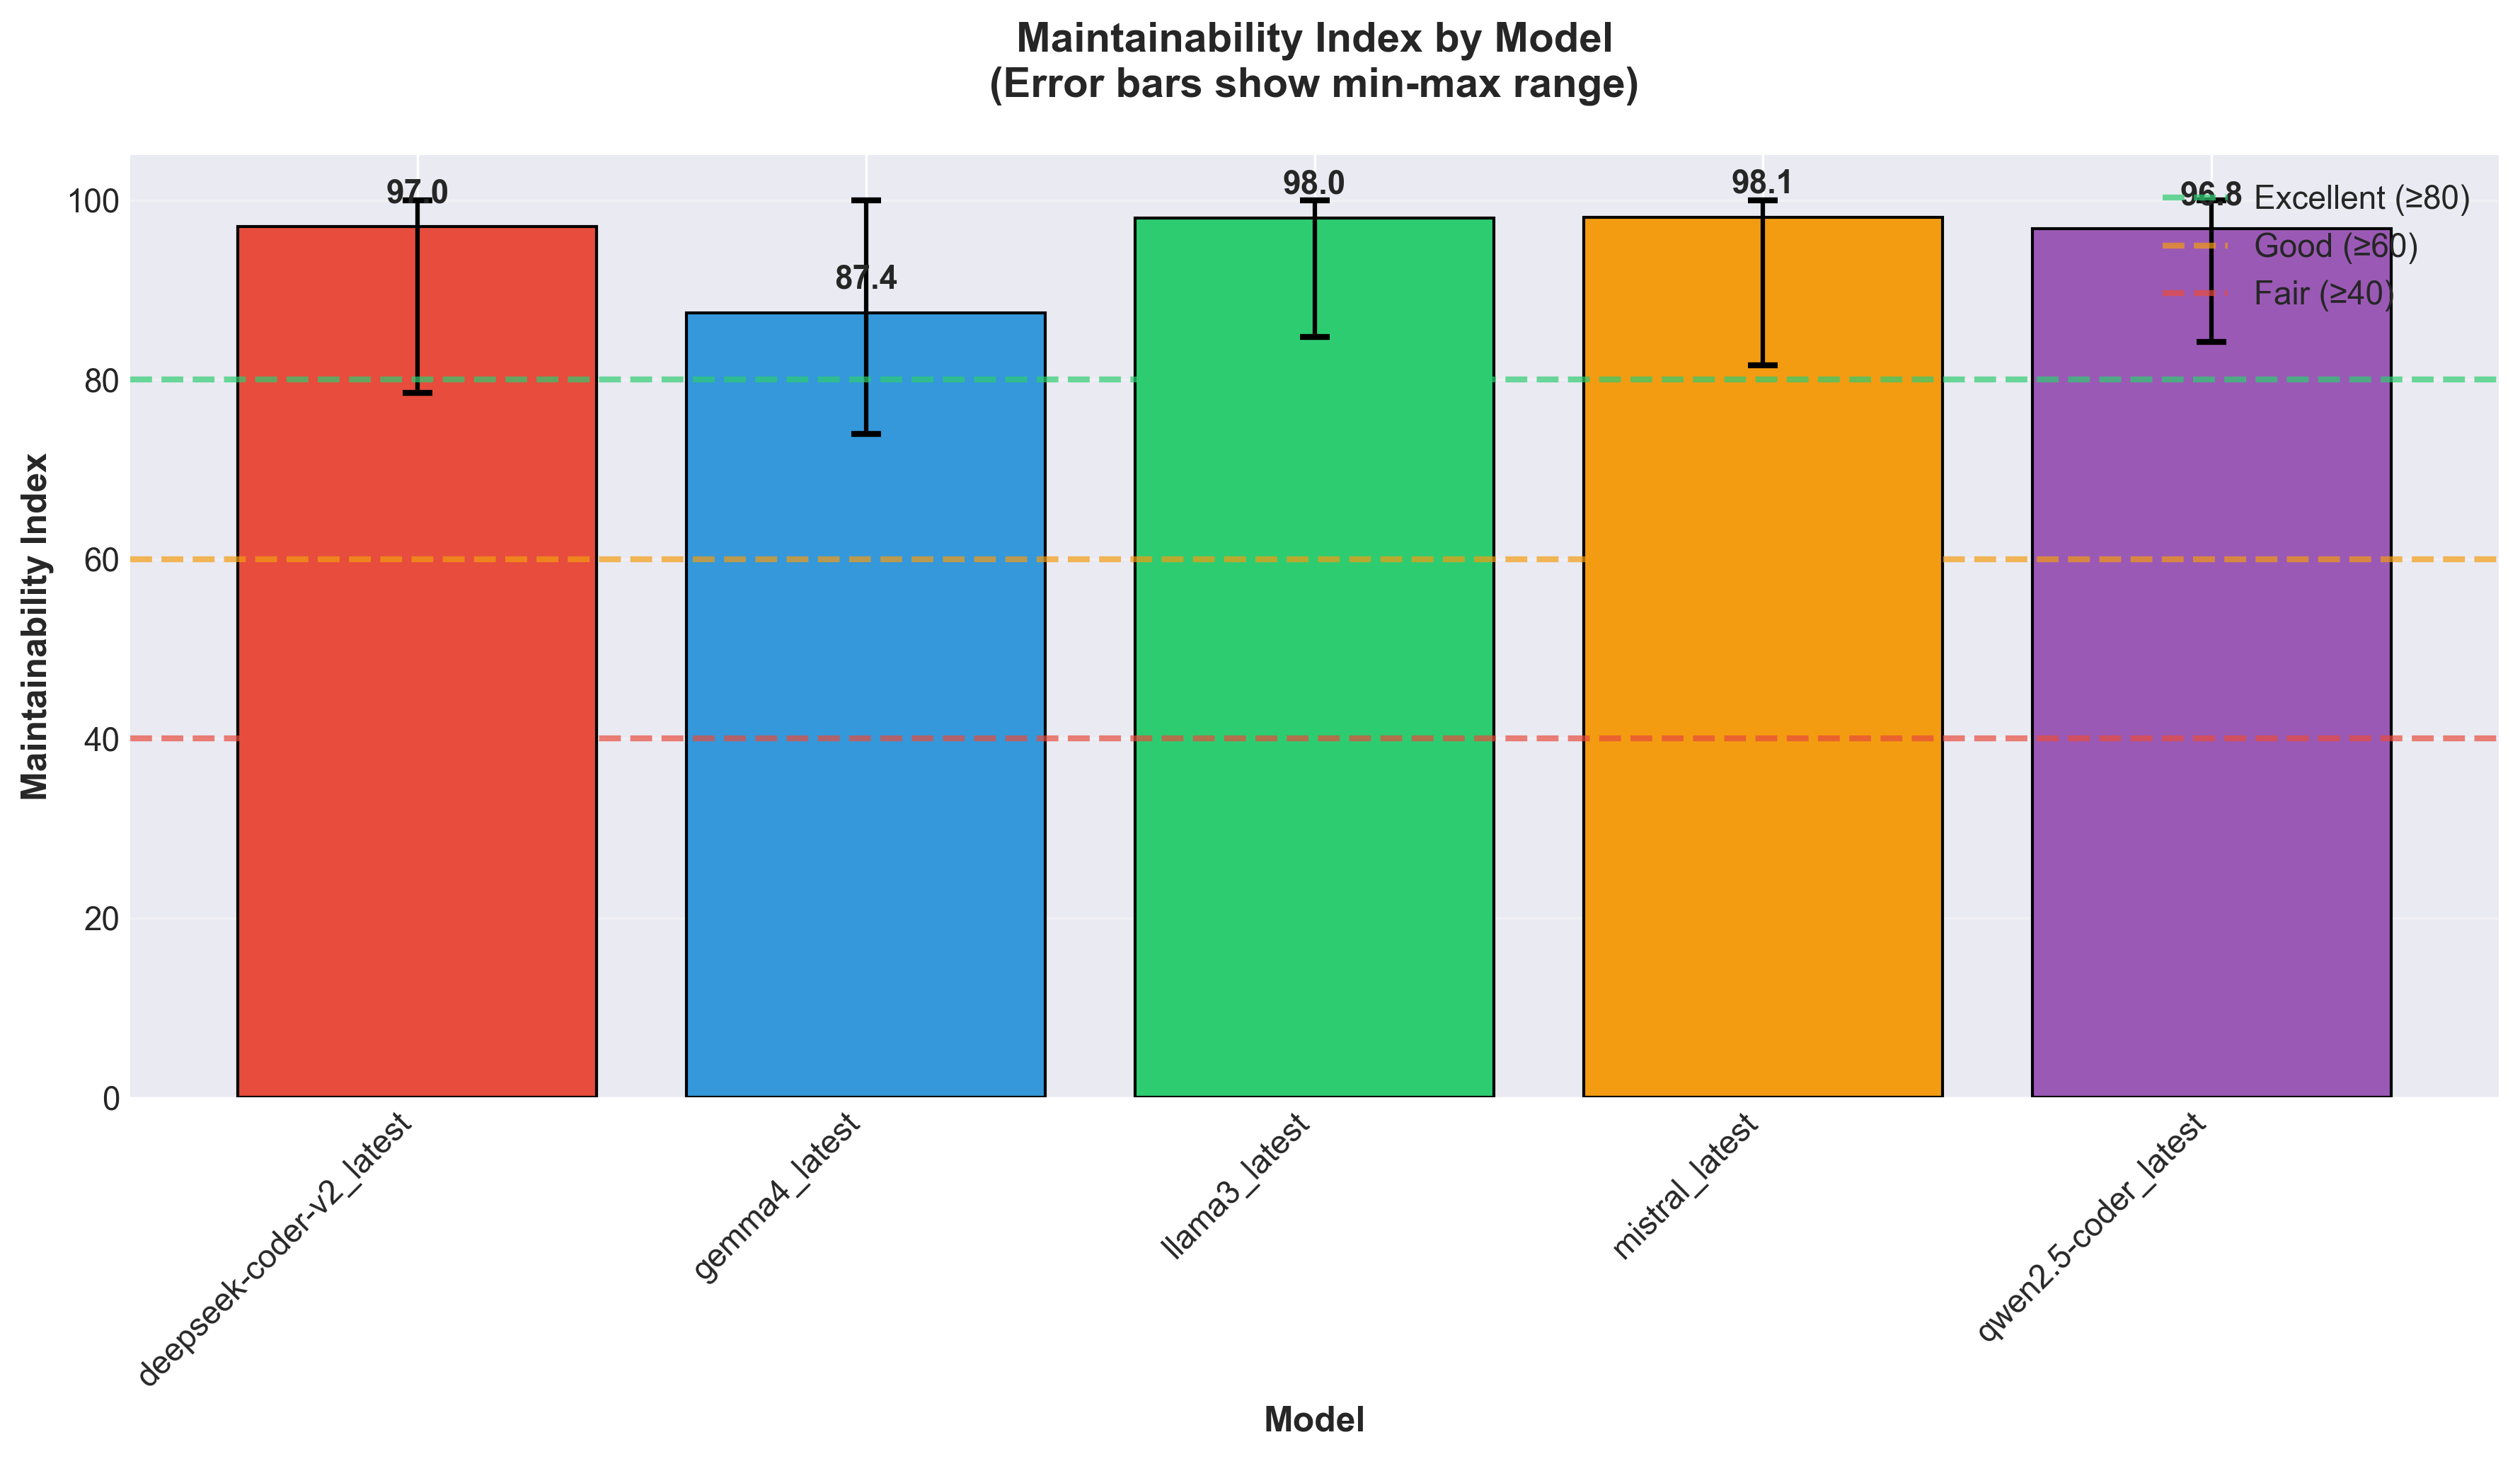
\includegraphics[width=0.9\linewidth]{images/03_maintainability.png}
    \caption{Onderhoudbaarheid van de gegenereerde code.}
    \label{fig:maintainability}
\end{figure}

\begin{figure}[htbp]
    \centering
    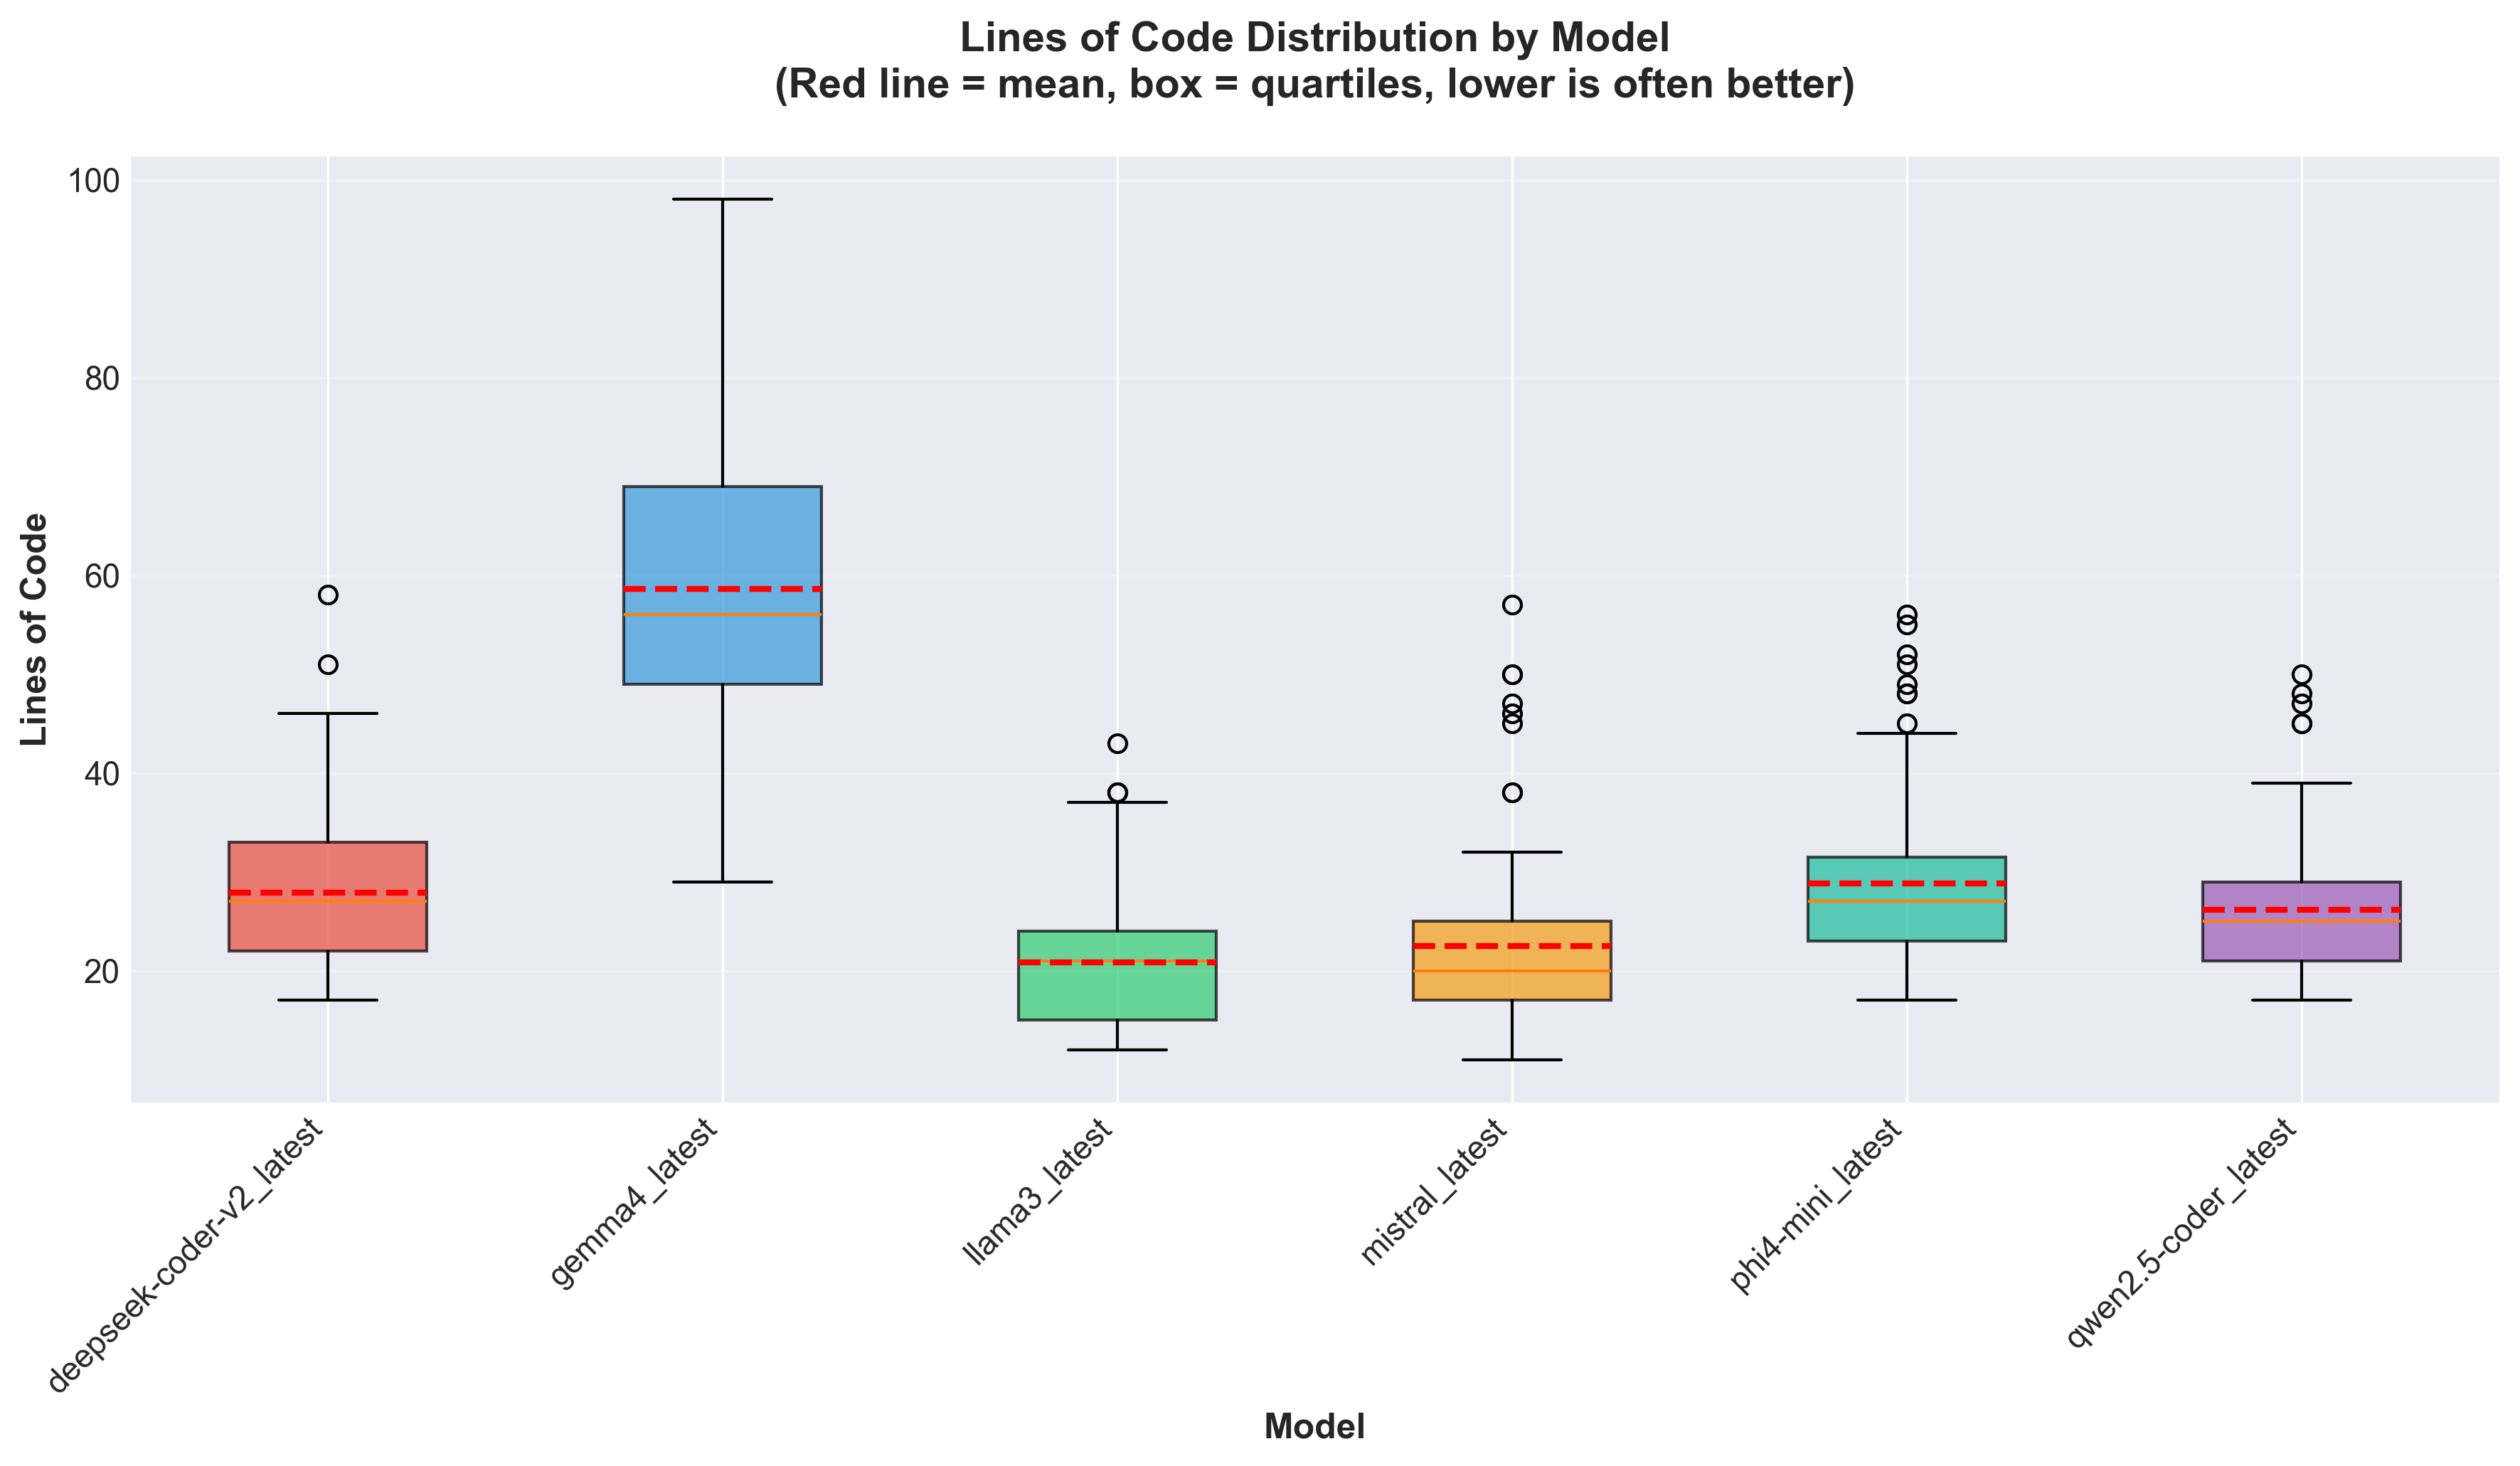
\includegraphics[width=0.9\linewidth]{images/04_lines_of_code.png}
    \caption{Aantal regels code per gegenereerde oplossing.}
    \label{fig:lines_of_code}
\end{figure}

\begin{figure}[htbp]
    \centering
    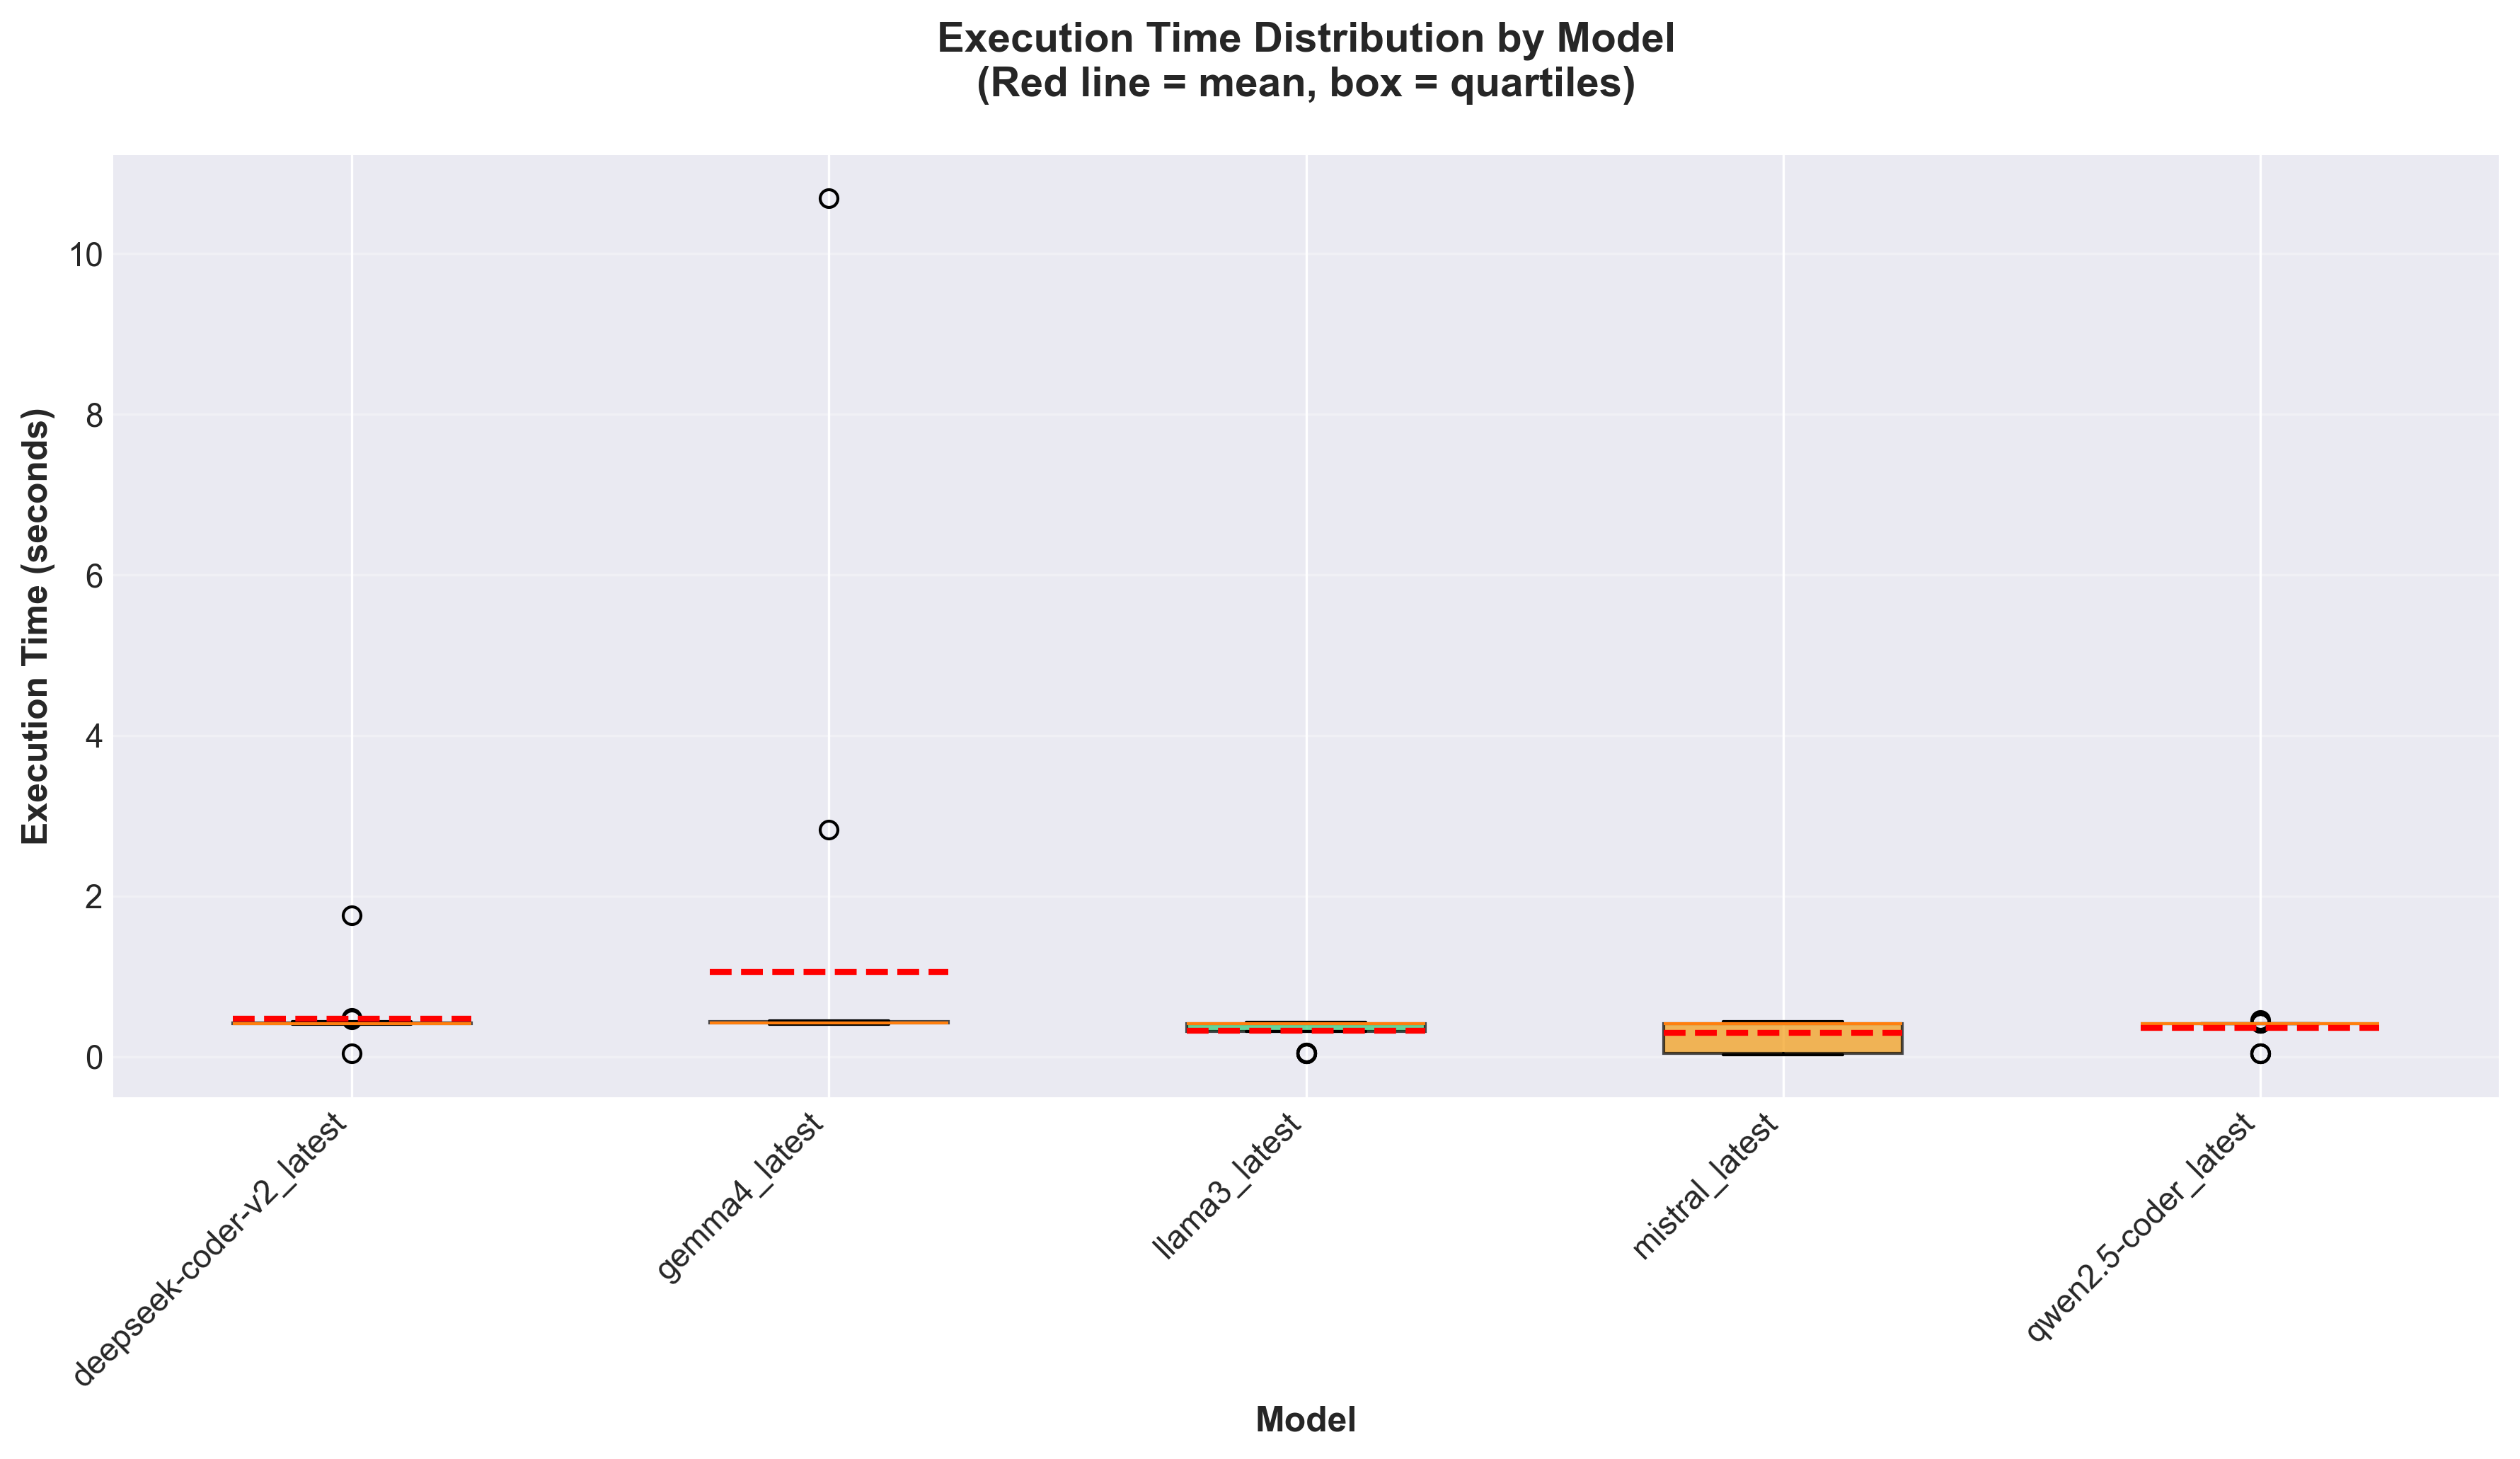
\includegraphics[width=0.9\linewidth]{images/05_execution_times.png}
    \caption{Uitvoeringstijden van de gegenereerde oplossingen.}
    \label{fig:execution_times}
\end{figure}

\begin{figure}[htbp]
    \centering
    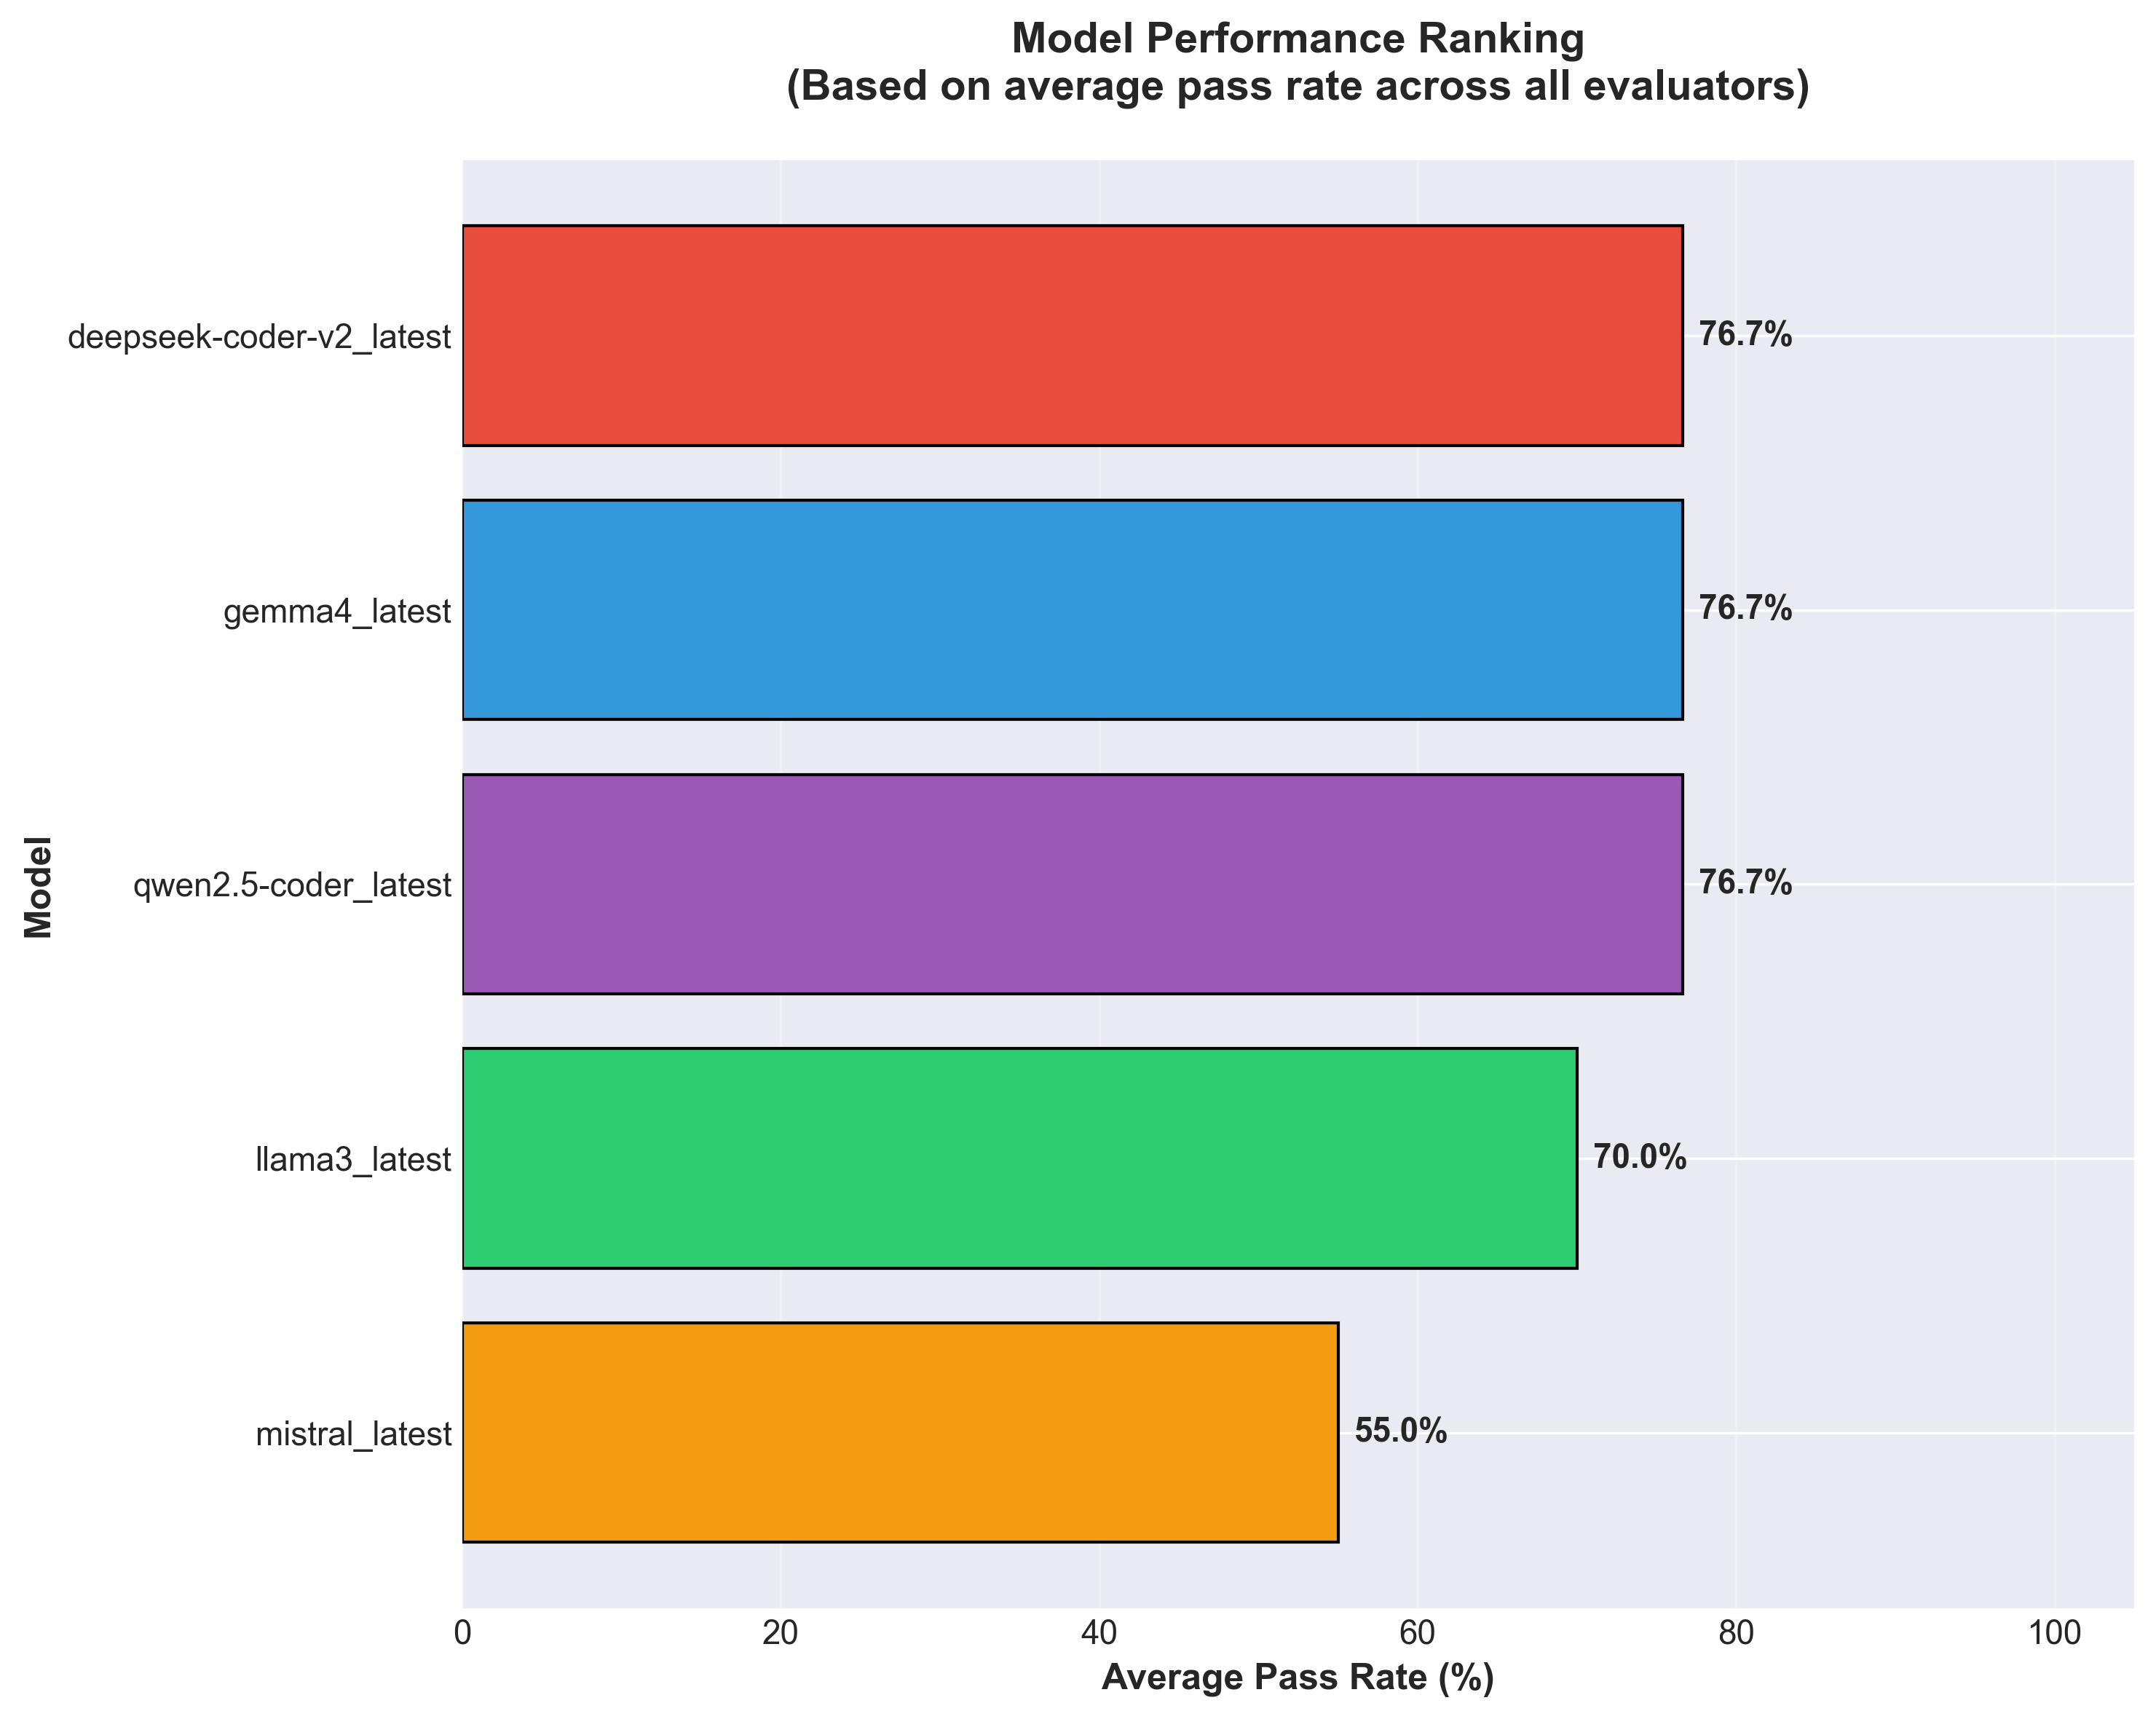
\includegraphics[width=0.9\linewidth]{images/07_model_ranking.png}
    \caption{Rangschikking van de modellen op basis van de overall prestatie.}
    \label{fig:model_ranking}
\end{figure}

\begin{figure}[htbp]
    \centering
    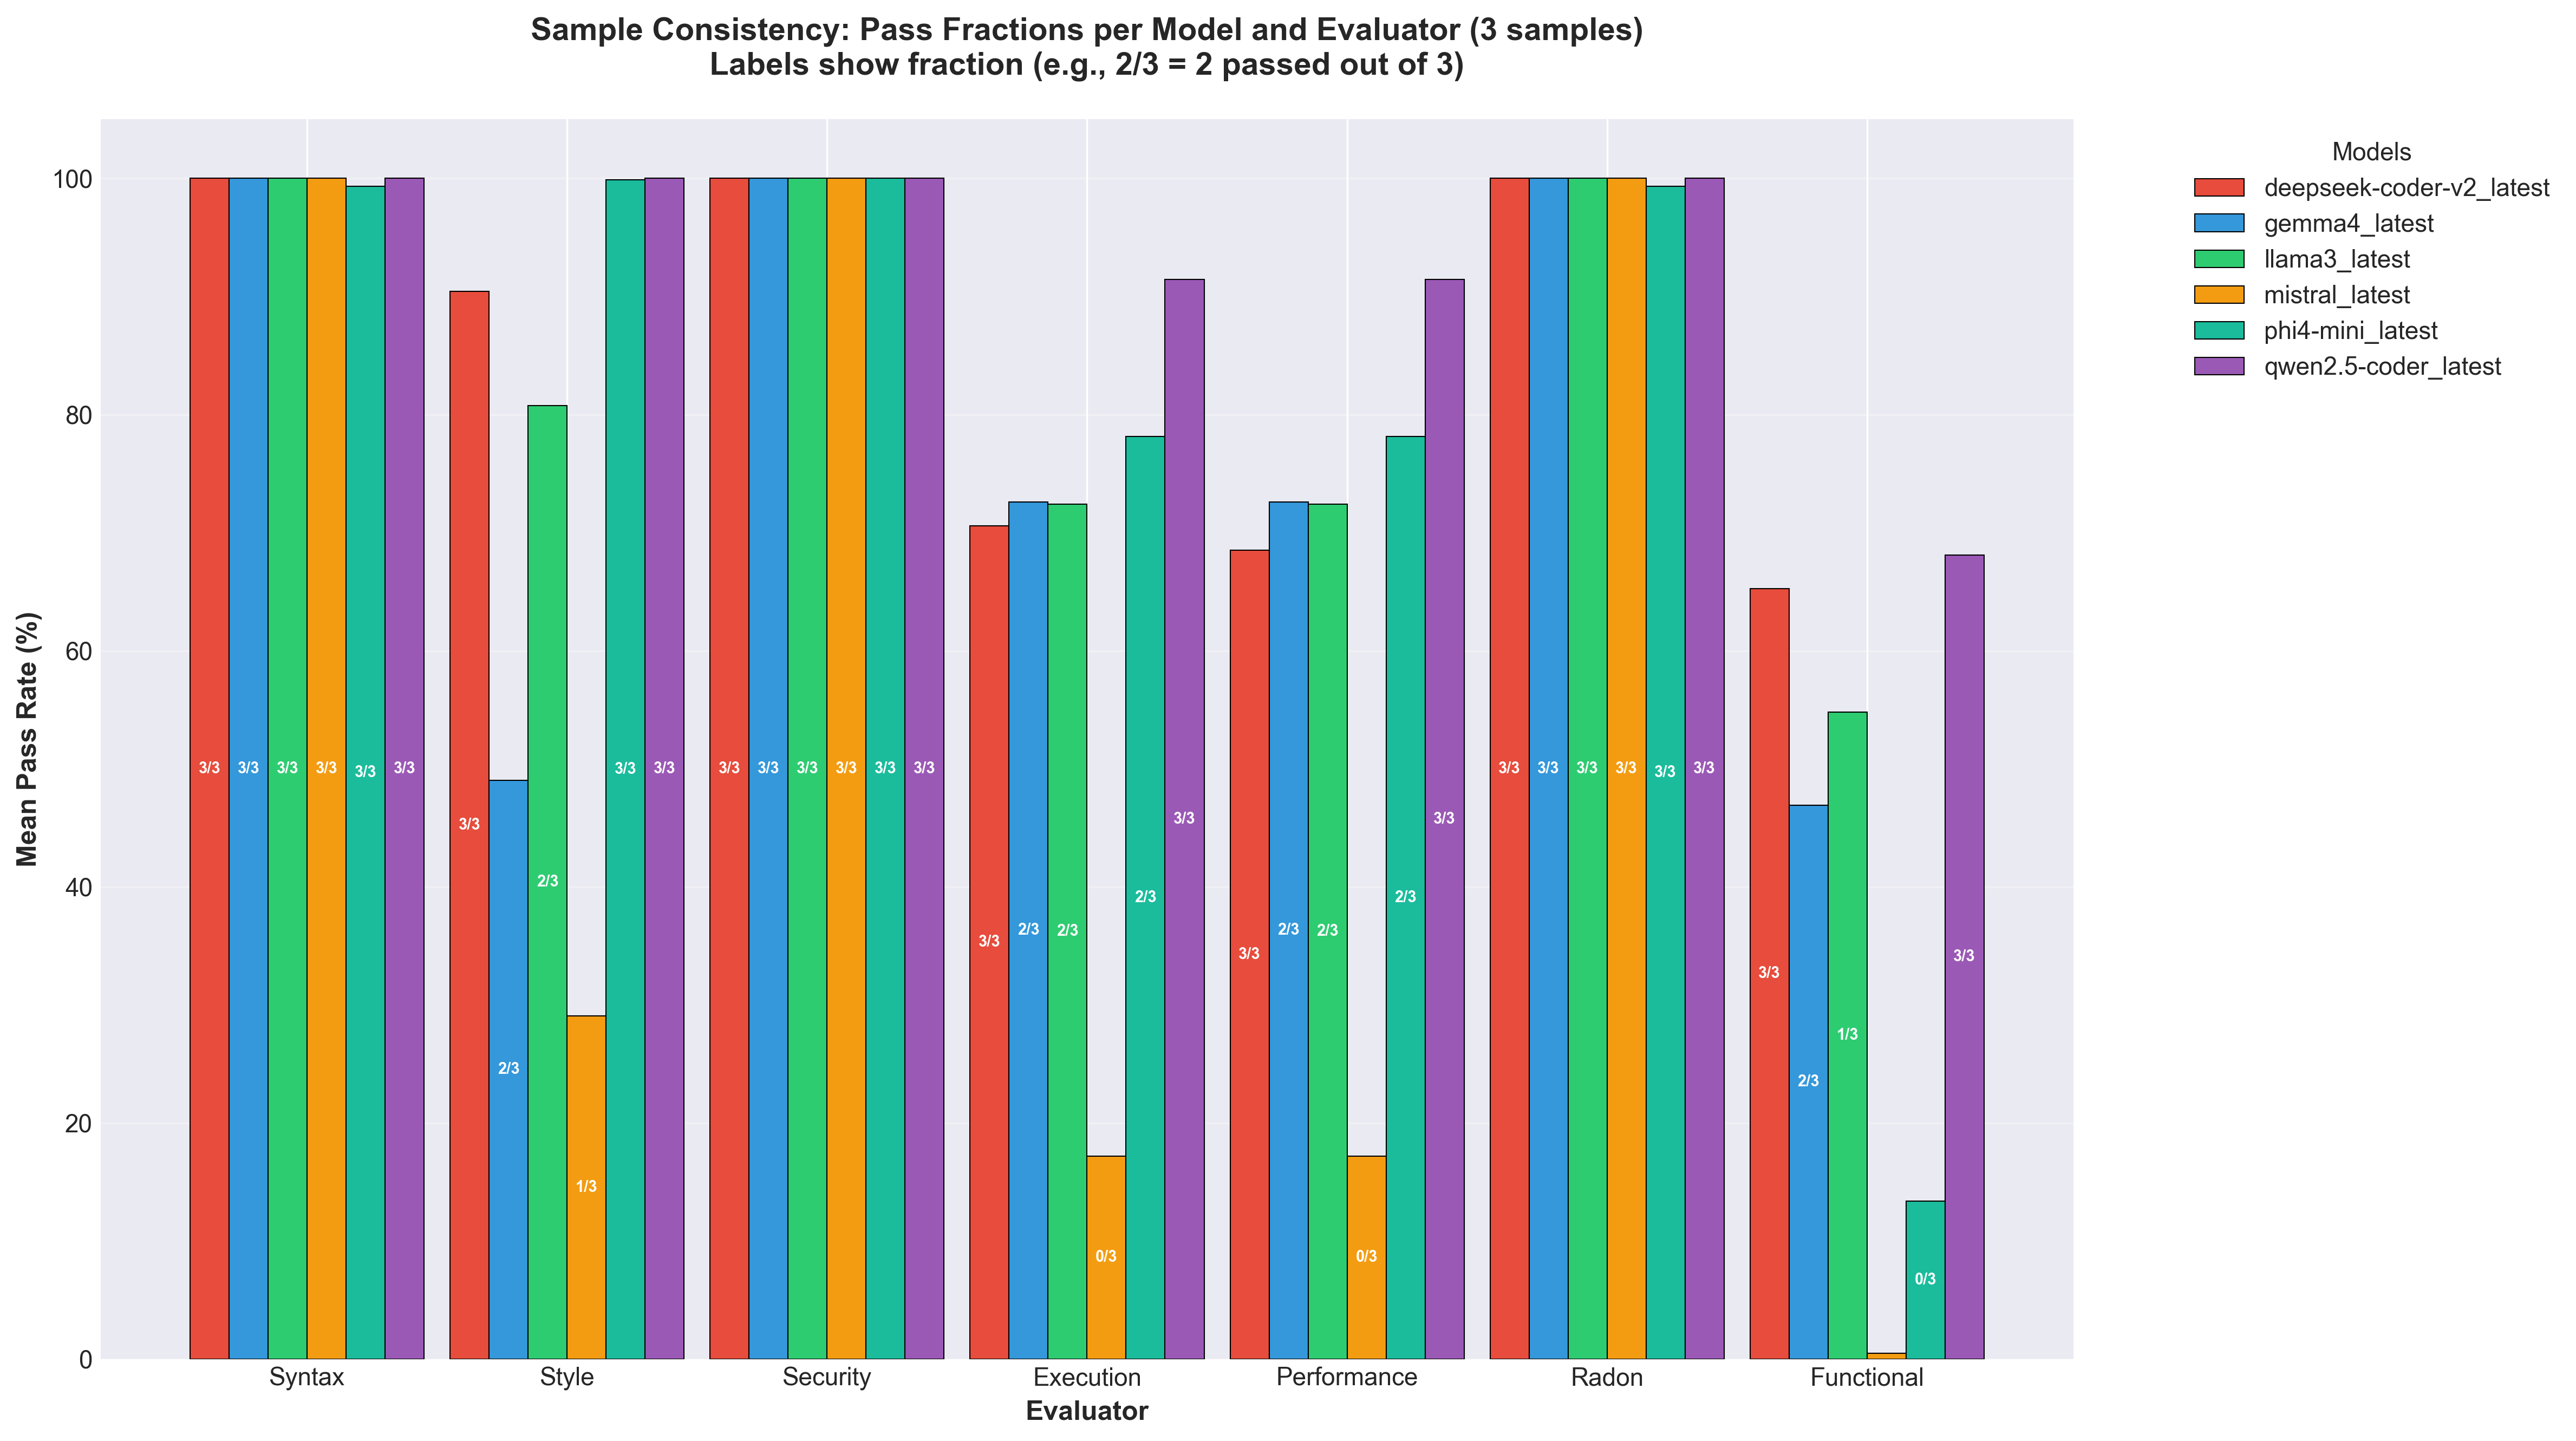
\includegraphics[width=0.9\linewidth]{images/08_sample_consistency.png}
    \caption{Consistentie van de samples per evaluator.}
    \label{fig:08_sample_consistency}
\end{figure}

\begin{figure}[htbp]
    \centering
    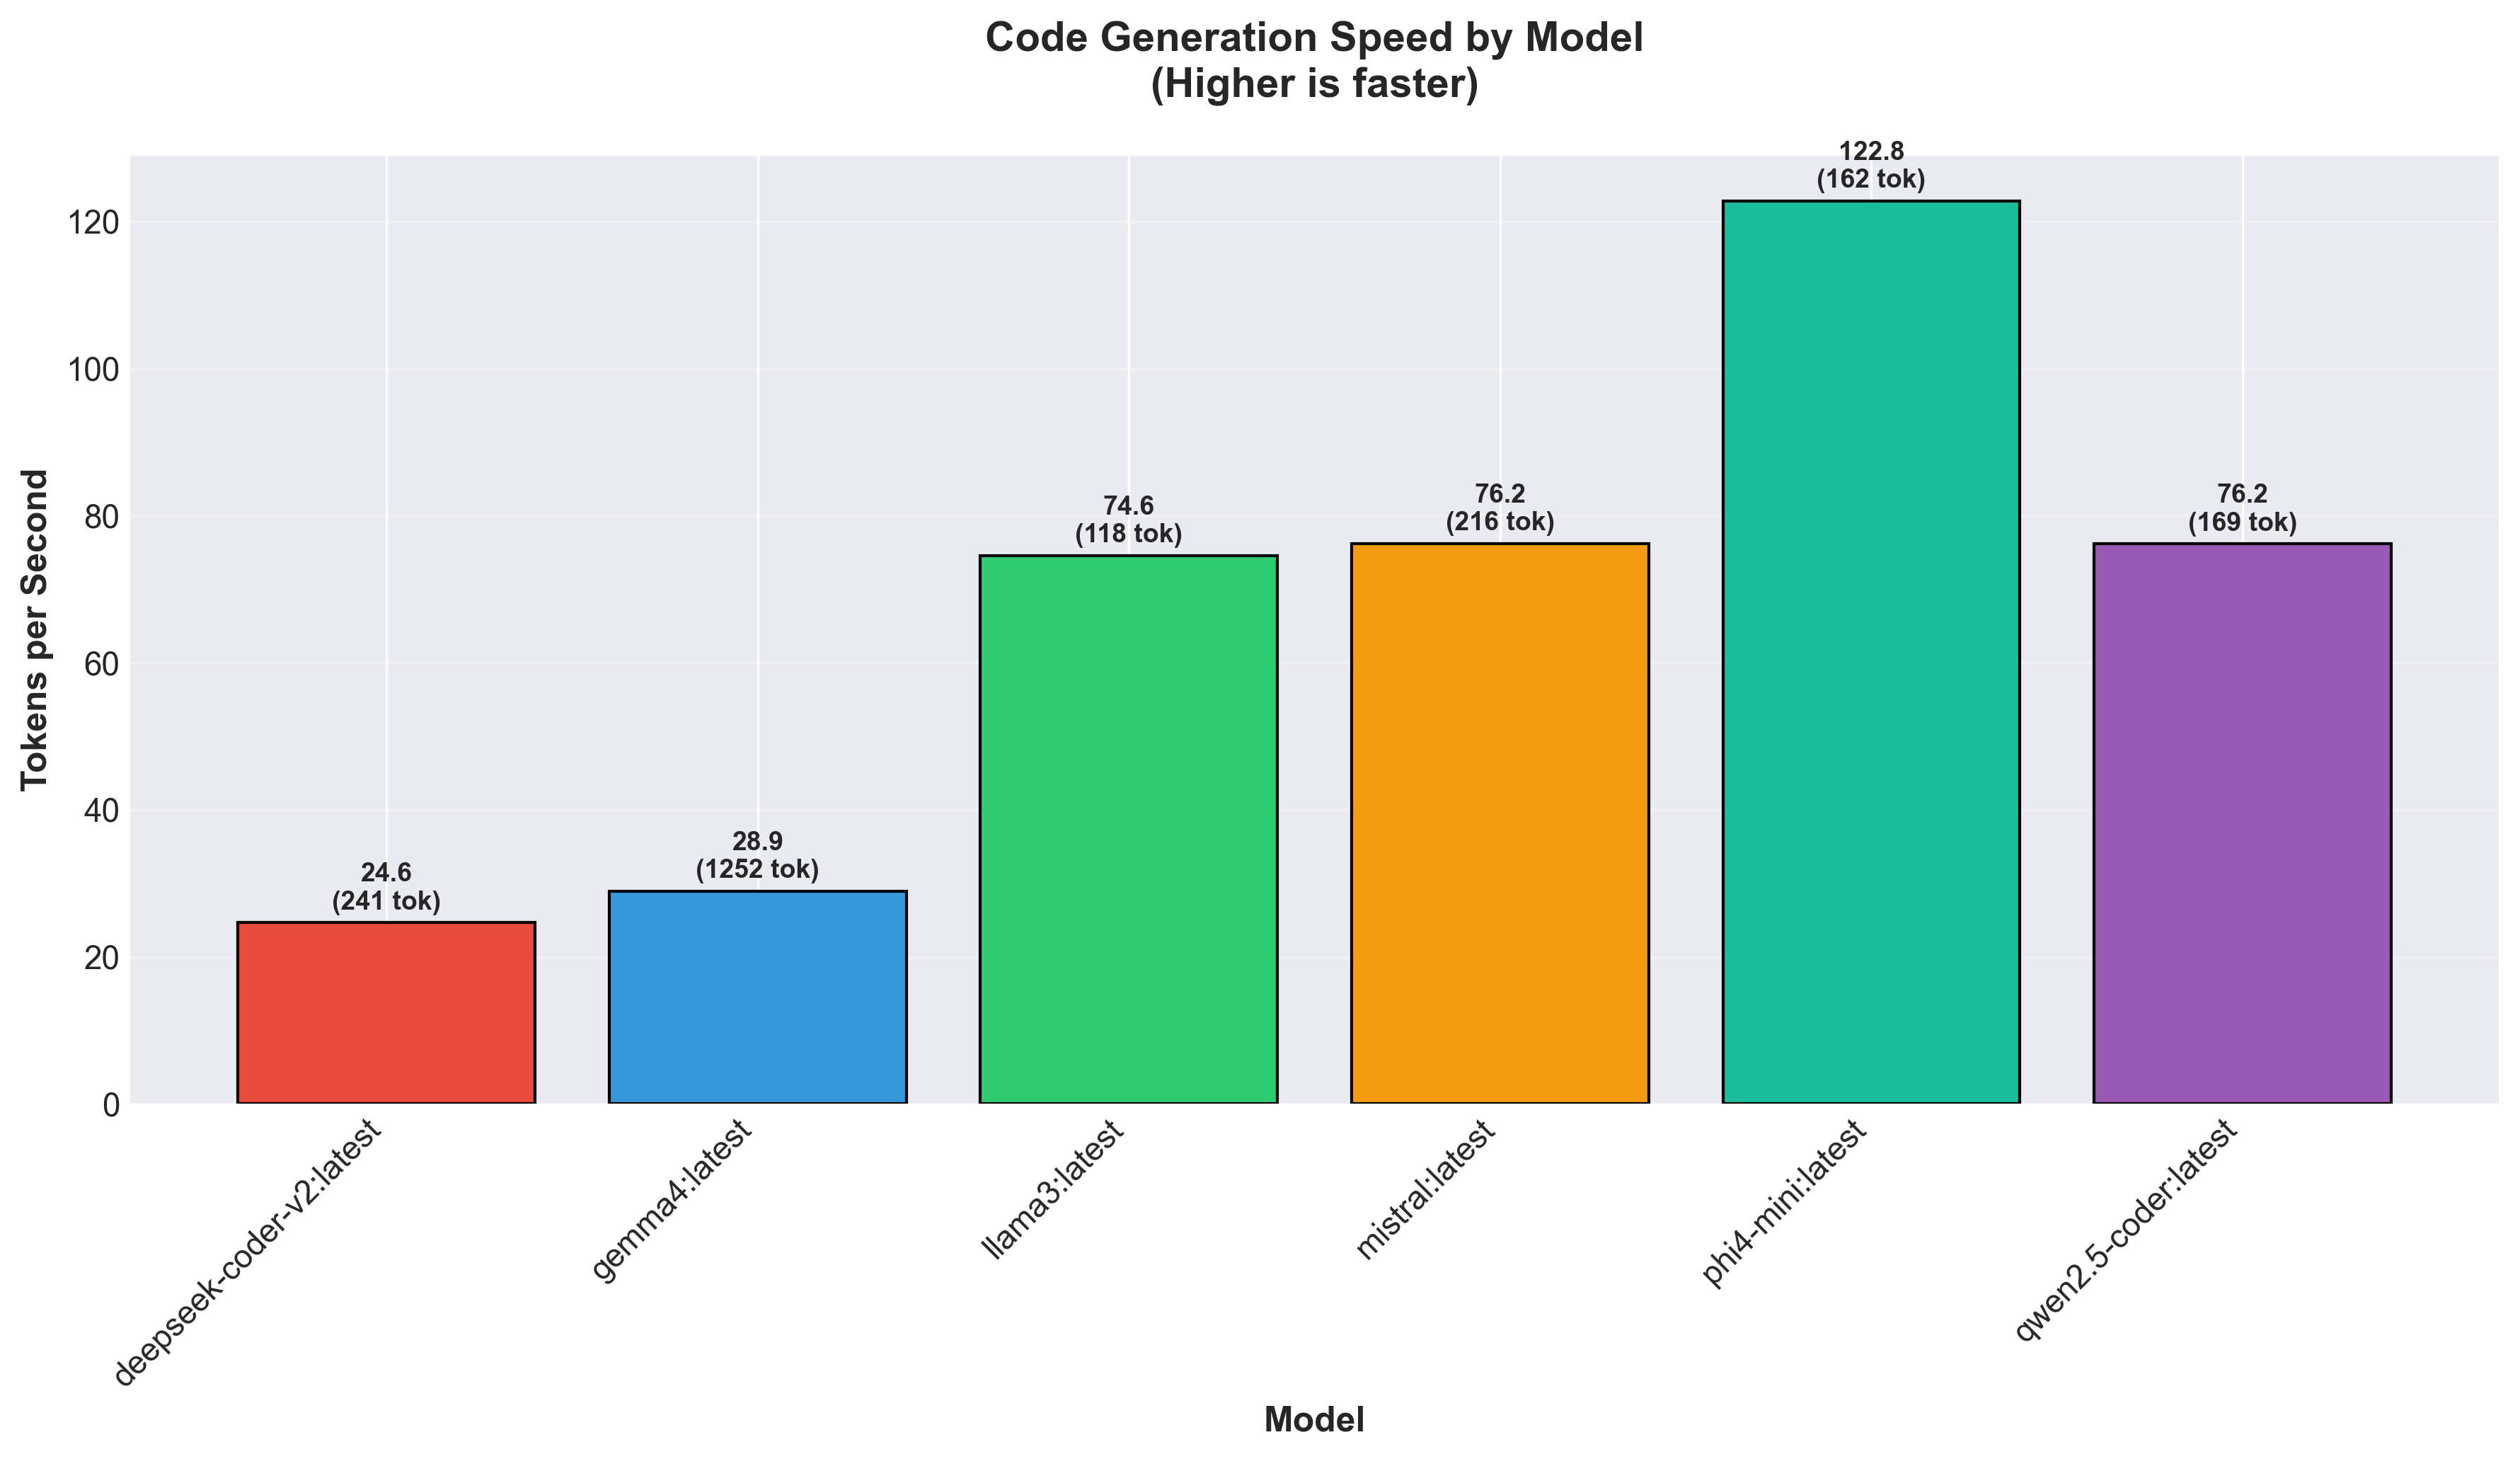
\includegraphics[width=0.9\linewidth]{images/09_generation_speed.png}
    \caption{Generatiesnelheid van de modellen.}
    \label{fig:09_generation_speed}
\end{figure}
